\documentclass[12pt,a4paper]{report}

% Package untuk margin
\usepackage[margin=1in]{geometry}

% Package untuk font Times New Roman
\usepackage{mathptmx}
\usepackage[T1]{fontenc}

% Package untuk spacing
\usepackage{setspace}
\onehalfspacing % 1.5 spacing

% Package untuk gambar
\usepackage{graphicx}

% Package untuk bahasa Indonesia
\usepackage[english,indonesian]{babel}

% Package untuk tabel
\usepackage{booktabs}
\usepackage{longtable}
\usepackage{multirow}
\usepackage[table]{xcolor}

% Package untuk enumerate kustom
\usepackage{enumitem}

% Package untuk csquotes (dibutuhkan oleh biblatex)
\usepackage{csquotes}

% Package untuk daftar pustaka (APA style)
\usepackage[style=authoryear,backend=biber,maxcitenames=2,maxbibnames=99,uniquelist=false,dashed=false,autolang=other,language=english]{biblatex}
\addbibresource{references.bib}

% Konfigurasi untuk format APA
\DeclareNameAlias{sortname}{family-given}
\DeclareFieldFormat{apacase}{#1}
\renewcommand*{\nameyeardelim}{\addcomma\space}
\DeclareFieldFormat[article]{title}{#1}
\DeclareFieldFormat[inproceedings]{title}{#1}

% Custom strings untuk et al. dan lainnya
\DefineBibliographyStrings{english}{%
  andothers = {\em et\addabbrvspace al\adddot},
  and = {and},
  in = {In},
  page = {p\adddot},
  pages = {pp\adddot}
}

% Pengaturan tambahan untuk format nama
\renewcommand*{\finalnamedelim}{\addspace\&\space}
\AtEveryBibitem{%
  \clearlist{language}%
}

% Package untuk hyperlink (optional, untuk navigasi PDF)
\usepackage[hidelinks]{hyperref}

% Package untuk formatting chapter
\usepackage{titlesec}

% Package untuk box
\usepackage{fancybox}

% Package untuk flowchart
\usepackage{tikz}
\usetikzlibrary{shapes.geometric, arrows.meta, positioning, fit, calc}

% Package untuk equation
\usepackage{amsmath}

% Format chapter
\titleformat{\chapter}[display]
  {\normalfont\fontsize{14}{16}\bfseries\centering}
  {\MakeUppercase{\chaptertitlename} \thechapter}
  {0pt}
  {\MakeUppercase}

% Spacing untuk chapter (before, after)
\titlespacing*{\chapter}{0pt}{20pt}{20pt}

% Format section
\titleformat{\section}
  {\normalfont\fontsize{12}{14}\bfseries}
  {\thesection}
  {1em}
  {}

% Format subsection
\titleformat{\subsection}
  {\normalfont\fontsize{12}{14}\bfseries}
  {\thesubsection}
  {1em}
  {}

% Hilangkan indentasi paragraf dan tambah jarak antar paragraf
\setlength{\parindent}{1.25cm}
\setlength{\parskip}{6pt}

% Ubah nama default ke bahasa Indonesia
\addto\captionsindonesian{%
  \renewcommand{\contentsname}{DAFTAR ISI}%
  \renewcommand{\listfigurename}{DAFTAR GAMBAR}%
  \renewcommand{\listtablename}{DAFTAR TABEL}%
  \renewcommand{\bibname}{DAFTAR PUSTAKA}%
  \renewcommand{\chaptername}{BAB}%
  \renewcommand{\appendixname}{LAMPIRAN}%
  \renewcommand{\figurename}{Gambar}%
  \renewcommand{\tablename}{Tabel}%
}

% ========================================
% KONFIGURASI PROPOSAL PENELITIAN
% Edit bagian ini sesuai dengan data Anda
% ========================================

% Informasi Umum
\newcommand{\judulPenelitian}{Desain dan Implementasi TathyaTest: Test Case Generator Otomatis untuk Pengujian Fungsional Aplikasi Web}
\newcommand{\bidangPenelitian}{Bidang Penelitian}
\newcommand{\jenisPenelitian}{Penelitian Reguler Kompetisi} % atau jenis lainnya
\newcommand{\nomorSPDIPA}{xxx/2026}
\newcommand{\lokasiPenelitian}{Lokasi Penelitian}
\newcommand{\lamaPenelitian}{Maret - Oktober 2026} % dalam bulan
\newcommand{\biayaDiusulkan}{9.000.000} % tanpa titik/koma
\newcommand{\bulanTahun}{Januari 2026}

% Ketua Peneliti
\newcommand{\ketuaNama}{Dian Hanifudin Subhi, S.Kom., M.Kom.}
\newcommand{\ketuaNIP}{198806102019031018}
\newcommand{\ketuaNIDN}{0010068807}
\newcommand{\ketuaJabatan}{Asisten Ahli}
\newcommand{\ketuaProdi}{Program Studi}
\newcommand{\ketuaHP}{085163736894}
\newcommand{\ketuaEmail}{dhanifudin@polinema.ac.id}

% Anggota Peneliti 1
\newcommand{\anggotaSatuNama}{Dika Rizki Yunianto, S.Kom., M.Kom.}
\newcommand{\anggotaSatuNIDN}{0006069202}

% Anggota Peneliti 2
\newcommand{\anggotaDuaNama}{Ridwan Rismanto, S.ST., M.Kom., Ph.D.}
\newcommand{\anggotaDuaNIDN}{0018038602}

% Anggota Peneliti 3
\newcommand{\anggotaTigaNama}{Usman Nurhasan, S.Kom., M.Kom.}
\newcommand{\anggotaTigaNIDN}{0023098604}

% Mahasiswa yang terlibat
\newcommand{\jumlahMahasiswa}{4}

% Mahasiswa 1
\newcommand{\mahasiswaSatuNama}{Mochamad Imam Hanafi}
\newcommand{\mahasiswaSatuNIM}{2241720151}

% Mahasiswa 2
\newcommand{\mahasiswaDuaNama}{Regita Delya Putri}
\newcommand{\mahasiswaDuaNIM}{2241720137}

% Mahasiswa 3
\newcommand{\mahasiswaTigaNama}{Putri Ayu Aliciawati}
\newcommand{\mahasiswaTigaNIM}{2241720132}

% Mahasiswa 4
\newcommand{\mahasiswaEmpatNama}{Elis Nurhidayati}
\newcommand{\mahasiswaEmpatNIM}{2241720035}

% Pejabat Pengesah
\newcommand{\kajurNama}{Nama Kajur/Kaprodi}
\newcommand{\kajurNIP}{000000000000000000}
\newcommand{\kajurJabatan}{Ketua Program Studi}
\newcommand{\kajurProdi}{Nama Program Studi}

\newcommand{\ketuaPPMNama}{Prof. Dr. Ratna Ika Putri, S.T., M.T.}
\newcommand{\ketuaPPMNIDN}{197710222000122001}

\newcommand{\direkturNama}{Ir. Supriatna Adhisuwignjo, S.T., M.T.}
\newcommand{\direkturNIDN}{197101081999031001}

\newcommand{\ppkNama}{Tjandra Dewi Wulandari, S.E., M.M.}
\newcommand{\ppkNIDN}{197509162003122002}

\newcommand{\tanggalPengesahan}{10 Maret 2026}

% ========================================
% AKHIR KONFIGURASI
% ========================================

\begin{document}

% Halaman Cover (tanpa nomor halaman)
\begin{titlepage}
    \pagenumbering{gobble} % Hilangkan nomor halaman

    % Box di pojok kanan atas
    \begin{flushright}
        \fbox{
            \parbox{0.3\textwidth}{
                \centering
                \small \jenisPenelitian
            }
        }
    \end{flushright}

    \vspace{-0.5cm}

    \begin{center}
        % Judul Proposal
        {\large \textbf{USULAN PENELITIAN TERAPAN}}

        \vspace{0.5cm}

        {\large \textbf{TENTANG}}

        \vspace{0.5cm}

        % Judul Penelitian (uppercase dan bold)
        {\Large \textbf{\MakeUppercase{\judulPenelitian}}}

        \vspace{1cm}

        % Informasi pendanaan
        {\normalsize Penelitian ini dibiayai dengan Dana DIPA Politeknik Negeri Malang}

        \vspace{0.3cm}

        {\normalsize Nomor: SP DIPA \nomorSPDIPA}

        \vspace{1.2cm}

        % Oleh
        {\normalsize \textbf{Oleh:}}

        \vspace{0.5cm}

        % Daftar Peneliti
        \begin{tabular}{c}
            \textbf{\ketuaNama} \\
            NIDN: \ketuaNIDN \\[0.3cm]
            \textbf{\anggotaSatuNama} \\
            NIDN: \anggotaSatuNIDN \\[0.3cm]
            \textbf{\anggotaDuaNama} \\
            NIDN: \anggotaDuaNIDN \\[0.3cm]
            \textbf{\anggotaTigaNama} \\
            NIDN: \anggotaTigaNIDN \\
        \end{tabular}

        \vfill

        % Logo
        
\includegraphics[width=0.25\textwidth]{images/logo.png}

        \vspace{0.5cm}

        % Nama Institusi
        {\large \textbf{POLITEKNIK NEGERI MALANG}}

        \vspace{0.3cm}

        % Bulan dan Tahun
        {\large \textbf{\MakeUppercase{\bulanTahun}}}
    \end{center}
\end{titlepage}

\clearpage

% Mulai penomoran romawi untuk halaman awal
\pagenumbering{roman}
\setcounter{page}{1}

% Halaman Pengesahan
\begin{center}
    {\Large \textbf{HALAMAN PENGESAHAN}}
\end{center}

\vspace{1cm}

\noindent
\begin{tabular}{@{}ll}
Judul Penelitian & : \judulPenelitian \\
Bidang Penelitian & : \bidangPenelitian \\
Ketua Peneliti & : \\
\quad a. Nama Lengkap & : \ketuaNama \\
\quad b. NIDN & : \ketuaNIDN \\
\quad c. Jabatan Fungsional & : \ketuaJabatan \\
\quad d. Program Studi & : \ketuaProdi \\
\quad e. Nomor HP & : \ketuaHP \\
\quad f. Alamat Email & : \ketuaEmail \\
Anggota Peneliti & : 3 orang \\
Mahasiswa yang Terlibat & : \jumlahMahasiswa{} orang \\
Lokasi Penelitian & : \lokasiPenelitian \\
Lama Penelitian & : \lamaPenelitian{} bulan \\
Biaya yang Diusulkan & : Rp \biayaDiusulkan \\
\end{tabular}

\vspace{2cm}

\begin{flushright}
    Malang, \tanggalPengesahan
\end{flushright}

\vspace{1cm}

\noindent
\begin{minipage}[t]{0.45\textwidth}
    \begin{center}
        Mengetahui,\\
        \kajurJabatan\\
        \kajurProdi

        \vspace{3cm}

        \textbf{\underline{\kajurNama}}\\
        NIP. \kajurNIP
    \end{center}
\end{minipage}
\hfill
\begin{minipage}[t]{0.45\textwidth}
    \begin{center}
        Ketua Peneliti

        \vspace{3cm}

        \textbf{\underline{\ketuaNama}}\\
        NIDN. \ketuaNIDN
    \end{center}
\end{minipage}

\vspace{1cm}

\begin{center}
    Menyetujui,\\
    Ketua P3M

    \vspace{3cm}

    \textbf{\underline{\ketuaPTMNama}}\\
    NIP. \ketuaPTMNIP
\end{center}

\clearpage

% Halaman Identitas dan Uraian Umum Penelitian
\chapter*{IDENTITAS DAN URAIAN UMUM PENELITIAN}
\addcontentsline{toc}{chapter}{IDENTITAS DAN URAIAN UMUM PENELITIAN}

\begin{enumerate}[itemsep=0.2cm]
\item Judul Penelitian: \judulPenelitian

\item Tim Peneliti:

\vspace{0.1cm}
{\small
\begin{longtable}{|c|p{3cm}|p{1.8cm}|p{2.5cm}|p{2.5cm}|p{1.3cm}|}
\hline
\textbf{No} & \textbf{Nama} & \textbf{Jabatan} & \textbf{Bidang Keahlian} & \textbf{Jurusan} & \textbf{Alokasi Waktu} \\
\hline
\endfirsthead
\hline
\textbf{No} & \textbf{Nama} & \textbf{Jabatan} & \textbf{Bidang Keahlian} & \textbf{Jurusan} & \textbf{Alokasi Waktu} \\
\hline
\endhead
1 & \ketuaNama\newline NIDN: \ketuaNIDN & Ketua & Rekayasa Perangkat Lunak & Teknik Informatika & 12 \\
\hline
2 & \anggotaSatuNama\newline NIDN: \anggotaSatuNIDN & Anggota 1 & Basis Data dan Sistem Informasi & Teknik Informatika & 10 \\
\hline
3 & \anggotaDuaNama\newline NIDN: \anggotaDuaNIDN & Anggota 2 & Kecerdasan Buatan dan Data Science & Teknik Informatika & 10 \\
\hline
4 & \anggotaTigaNama\newline NIDN: \anggotaTigaNIDN & Anggota 3 & Jaringan Komputer dan Sistem Terdistribusi & Teknik Informatika & 10 \\
\hline
5 & \mahasiswaSatuNama\newline NIM: \mahasiswaSatuNIM & Pembantu pelaksana & Teknik Informatika & Teknik Informatika & 8 \\
\hline
6 & \mahasiswaDuaNama\newline NIM: \mahasiswaDuaNIM & Pembantu pelaksana & Teknik Informatika & Teknik Informatika & 8 \\
\hline
7 & \mahasiswaTigaNama\newline NIM: \mahasiswaTigaNIM & Pembantu pelaksana & Teknik Informatika & Teknik Informatika & 8 \\
\hline
8 & \mahasiswaEmpatNama\newline NIM: \mahasiswaEmpatNIM & Pembantu pelaksana & Teknik Informatika & Teknik Informatika & 8 \\
\hline
\end{longtable}
}

\item Objek Penelitian: Aplikasi berbasis web menggunakan dataset internal Jurusan Teknologi Informasi sebagai studi kasus.

\item Masa Pelaksanaan: \lamaPenelitian\ bulan (\bulanTahun)

\item Biaya yang Diusulkan: Rp \biayaDiusulkan,-

\item Lokasi Penelitian: Jurusan Teknologi Informasi, Politeknik Negeri Malang

\item Instansi Lain yang Terlibat: Tidak ada

\item Temuan yang Ditargetkan (TKT): Prototipe TathyaTest dengan target TKT 4, yaitu validasi komponen dalam lingkungan laboratorium. TathyaTest sudah dapat digunakan untuk pengujian aplikasi web dengan dataset internal, meskipun masih dalam skala terbatas.

\item Kontribusi Mendasar pada Suatu Bidang Ilmu: Penelitian ini memberikan kontribusi pada bidang Software Testing dan Quality Assurance melalui pengembangan metode otomatis untuk test case generation yang memanfaatkan web crawling dan ekstraksi elemen HTML. TathyaTest mengotomatisasi proses ini dengan memanfaatkan dataset internal untuk menghasilkan test case yang lebih relevan dan kontekstual.

\item Jurnal Ilmiah yang Menjadi Sasaran: Jurnal nasional terakreditasi Sinta 3 Sisfokom pada bidang Teknologi Informasi.

\item Rencana Luaran HKI: Hak Cipta untuk prototipe TathyaTest dengan status Granted.

\end{enumerate}

\clearpage

% Daftar Isi
\tableofcontents
\clearpage

% Ringkasan
\chapter*{RINGKASAN}
\addcontentsline{toc}{chapter}{RINGKASAN}

Pengujian aplikasi web di Jurusan Teknologi Informasi Politeknik Negeri Malang menghadapi tantangan dalam memastikan kualitas aplikasi akademik seperti Kompen, Jayanti, dan Whistleblower. Alat automation testing seperti Selenium, Cypress, dan Playwright masih memerlukan pembuatan test case manual yang menjadi bottleneck. TathyaTest hadir sebagai test case generator otomatis yang mengintegrasikan web crawling (Colly), ekstraksi HTML (Goquery), dan dataset internal aplikasi untuk menghasilkan test case relevan dan kontekstual. Penelitian ini mengukur efektivitas TathyaTest dalam menghasilkan test case otomatis, meningkatkan cakupan pengujian fungsional (CRUD, autentikasi, akses modul), dan validasi ekspektasi berdasarkan dataset internal. Metode Prototyping digunakan secara iteratif dari prototipe CRUD sederhana, perbaikan berdasarkan umpan balik, hingga integrasi Playwright untuk cross-browser testing (Chrome, Firefox, WebKit) dengan dataset aplikasi internal. Penelitian dibatasi pada aplikasi web MVC dengan fokus pengujian fungsional berbasis UI. Analisis data menggunakan pendekatan kuantitatif (test coverage, efisiensi waktu, akurasi deteksi bug). Luaran meliputi prototipe TathyaTest TKT 4, publikasi jurnal Sinta 3, dan Hak Cipta. Penelitian ini berkontribusi pada Software Testing dan Quality Assurance melalui metode otomatis test case generation berbasis web crawling dan ekstraksi HTML, menjadi pondasi roadmap lima tahun pengembangan TathyaTest dengan integrasi AI dan machine learning.

\vspace{0.5cm}

\noindent
\textbf{Kata Kunci:} automation testing, test case generation, web crawling, functional testing, Playwright 

\clearpage

% Mulai penomoran arabic dari Bab 1
\pagenumbering{arabic}
\setcounter{page}{1}

% Bab 1: Pendahuluan
\chapter{PENDAHULUAN}\label{bab-i-pendahuluan}

\section{Latar Belakang}\label{latar-belakang}

Perkembangan pesat dalam teknologi informasi telah memberikan dampak besar pada berbagai sektor, termasuk dunia pendidikan. Di perguruan tinggi, aplikasi berbasis web telah menjadi alat penting dalam menyelenggarakan kegiatan akademik dan administrasi, seperti sistem manajemen akademik, pengelolaan keuangan, dan pelaporan data. Di Jurusan Teknologi Informasi, aplikasi-aplikasi seperti Kompen, Jayanti, dan Whistleblower digunakan oleh mahasiswa, dosen, dan staf untuk kegiatan yang sangat krusial. Aplikasi-aplikasi tersebut menjadi motivasi awal penelitian ini, meskipun demikian tantangan utama yang dihadapi berlaku umum bagi setiap aplikasi web dengan kontrol akses berbasis peran (role-based access control/RBAC) \parencite{sandhu1996rbac}: memastikan aplikasi tersebut berfungsi dengan baik dan selalu tersedia tanpa gangguan.

Gangguan dalam ketersediaan aplikasi atau kesalahan dalam fungsionalitas dapat menurunkan kualitas layanan dan berdampak pada pengalaman pengguna. Pemantauan ketersediaan server secara konvensional (misalnya status HTTP 200) tidak dapat memastikan bahwa fungsi inti aplikasi -- seperti proses login, penegakan RBAC, validasi input, maupun operasi CRUD -- benar-benar berjalan sebagaimana mestinya; sebuah aplikasi dapat ``tersedia'' secara jaringan namun gagal secara fungsional. Oleh karena itu, penting bagi aplikasi-aplikasi berbasis web di Jurusan Teknologi Informasi untuk selalu diuji secara fungsional secara berkala guna memastikan bahwa mereka berfungsi sesuai dengan yang diharapkan dan siap digunakan setiap saat.

Salah satu metode yang paling efektif untuk memastikan kualitas aplikasi perangkat lunak adalah dengan menggunakan automation testing. Dalam pengembangan perangkat lunak modern, automated testing telah menjadi praktik penting yang menawarkan berbagai peluang sekaligus tantangan yang perlu dinavigasi dengan baik \parencite{solige2025automation}. Automation testing menawarkan berbagai keuntungan, termasuk penghematan waktu, pengurangan kesalahan manusia, dan kemampuan untuk menjalankan pengujian secara berulang tanpa menambah biaya yang signifikan. Systematic mapping study menunjukkan bahwa automated testing untuk aplikasi web telah menjadi area penelitian yang berkembang pesat dengan berbagai pendekatan dan teknik yang terus diperbarui \parencite{wang2023}. Dalam konteks pengujian aplikasi berbasis web, penggunaan alat automation testing sangat berguna untuk menguji berbagai skenario pengguna dan fungsionalitas aplikasi secara cepat dan akurat.

Namun, meskipun terdapat berbagai alat untuk automation testing seperti Selenium, Cypress, dan Playwright, tantangan terbesar adalah bagaimana mengotomatisasi pembuatan test case yang relevan dengan fungsionalitas aplikasi yang diuji. Software testability yang tinggi memfasilitasi proses pengujian yang lebih efektif, namun banyak aplikasi web yang masih memiliki testability yang rendah \parencite{garousi2019testability}. Meskipun berbagai alat pengujian otomatis ada, kebanyakan dari alat ini masih memerlukan input manual untuk mendefinisikan skenario pengujian, yang pada gilirannya menambah waktu dan beban kerja pengujian. Beberapa penelitian juga menekankan pentingnya otomatisasi dalam test case generation untuk aplikasi web, di mana pendekatan otomatis dapat secara signifikan mengurangi effort manual dan meningkatkan coverage pengujian \parencite{leotta2021,romano2022}. Oleh karena itu, diperlukan sebuah solusi yang dapat mengotomatisasi test case generation secara efisien untuk memastikan bahwa pengujian dilakukan secara lebih cepat dan lebih menyeluruh.

TathyaTest: Test Case Generator Otomatis merupakan solusi yang direncanakan untuk mengatasi masalah ini. TathyaTest dirancang untuk menghasilkan test case otomatis dengan melakukan crawling pada DOM (Document Object Model) aplikasi yang telah dirender oleh browser menggunakan Playwright, sehingga mampu menjelajahi aplikasi modern berbasis single-page application (SPA) sekalipun. Dengan membangun model elemen dan matriks akses per peran pengguna (RBAC) secara otomatis dari hasil crawling, TathyaTest direncanakan dapat menghasilkan test case fungsional yang relevan dan kontekstual untuk berbagai aplikasi berbasis web, sehingga pengujian dapat dilakukan dengan lebih cepat dan lebih komprehensif. Literature review mengenai pendekatan test case generation menunjukkan berbagai teknik yang dapat digunakan untuk mengotomatisasi pembuatan test case, yang membantu mengidentifikasi bug lebih cepat dan meningkatkan cakupan pengujian \parencite{setiani2019,sahoo2021}. Pengalaman deployment automation testing di skala industri, seperti implementasi search-based software engineering dengan Sapienz di Facebook, membuktikan bahwa automated testing dapat memberikan nilai praktis yang signifikan dalam lingkungan produksi \parencite{alshahwan2018}. Hal ini sejalan dengan tujuan pengembangan TathyaTest, yang tidak hanya mengotomatiskan pembuatan test case tetapi juga meningkatkan efisiensi pengujian di Jurusan Teknologi Informasi.

Dengan adanya TathyaTest, proses pengujian dapat dilakukan secara lebih efisien, mengurangi ketergantungan pada pengujian manual yang memakan waktu dan sering kali tidak lengkap. Selain itu, TathyaTest akan memberikan manfaat yang signifikan dalam mempermudah pengujian aplikasi berbasis web, khususnya di lingkungan pendidikan tinggi, dengan memfokuskan pada pengujian fungsional aplikasi yang digunakan oleh mahasiswa dan dosen di Jurusan Teknologi Informasi. Penelitian ini diharapkan dapat memberikan kontribusi besar dalam meningkatkan kualitas aplikasi yang digunakan di perguruan tinggi dan memberikan dasar yang kuat bagi pengembangan alat pengujian perangkat lunak otomatis di masa depan.

\section{Rumusan Masalah}\label{rumusan-masalah}

\begin{enumerate}
    \item Bagaimana efektivitas TathyaTest dalam menghasilkan test case otomatis untuk pengujian aplikasi berbasis web beserta kemampuannya dalam mendeteksi cacat fungsional, pada aplikasi berarsitektur MVC dan RBAC?
    \item Sejauh mana TathyaTest dapat meningkatkan cakupan pengujian aplikasi berbasis web, diukur dari cakupan model elemen (form, field, navigasi, matriks RBAC) dan cakupan rute yang dihasilkan dari crawling DOM ter-render?
    \item Bagaimana TathyaTest dapat memvalidasi ekspektasi fungsional aplikasi berbasis web -- seperti memastikan login berhasil, data dapat disimpan, dan modul dapat diakses sesuai peran pengguna -- secara konsisten dan andal lintas browser?
\end{enumerate}

\section{Batasan Masalah}\label{batasan-masalah}

Untuk memfokuskan penelitian dan memastikan hasil yang optimal, batasan masalah dalam penelitian ini meliputi:

\begin{enumerate}
    \item Penelitian ini terbatas pada aplikasi berbasis web dengan arsitektur MVC (Model-View-Controller).
    \item Pengujian difokuskan pada fungsionalitas aplikasi yang mencakup operasi CRUD (Create, Read, Update, Delete), autentikasi pengguna, dan akses modul.
    \item Fitur halaman login tidak menerapkan mekanisme CAPTCHA atau autentikasi multi-faktor (MFA) yang dapat menghambat proses otomatisasi pengujian.
    \item Evaluasi direncanakan pada aplikasi studi kasus dengan arsitektur MVC dan RBAC (aplikasi Laravel berbasis Blade dan aplikasi Laravel berbasis Inertia-React) serta satu aplikasi eksternal (SauceDemo) sebagai pembanding (baseline); perluasan pengujian pada aplikasi internal Jurusan Teknologi Informasi (Kompen, Jayanti, Whistleblower) direncanakan sebagai tahap penelitian lanjutan.
    \item TathyaTest hanya menghasilkan test case untuk pengujian fungsional berbasis UI (User Interface) dan tidak mencakup pengujian non-fungsional seperti performance testing, security testing, atau load testing.
    \item Pengujian dilakukan pada browser modern (Chrome, Firefox, dan WebKit) menggunakan Playwright sebagai automation testing framework.
    \item Penelitian ini tidak mencakup pengujian untuk aplikasi mobile native atau aplikasi desktop.
\end{enumerate}

\section{Tujuan Penelitian}\label{tujuan-penelitian}

\begin{enumerate}
    \item Mengukur efektivitas TathyaTest dalam menghasilkan test case otomatis dan mendeteksi cacat fungsional (skor mutasi), dengan mengevaluasinya pada aplikasi studi kasus yang memiliki arsitektur MVC dan RBAC.
    \item Menilai seberapa baik TathyaTest dapat meningkatkan cakupan pengujian aplikasi berbasis web, diukur dari cakupan model elemen (form, field, navigasi, matriks RBAC) dan cakupan rute hasil crawling DOM ter-render.
    \item Mengevaluasi apakah TathyaTest dapat memvalidasi ekspektasi fungsional aplikasi berbasis web secara konsisten lintas browser, seperti memastikan login berhasil, data dapat disimpan, dan modul dapat diakses dengan benar sesuai peran pengguna.
\end{enumerate}

\section{Manfaat Penelitian}\label{manfaat-penelitian}

\begin{enumerate}
    \item Meningkatkan efisiensi pengujian perangkat lunak melalui otomatisasi pembuatan test case yang mengurangi ketergantungan pada pengujian manual.
    \item Meningkatkan cakupan pengujian dengan memastikan lebih banyak skenario diuji, termasuk yang mungkin terlewat dalam pengujian manual.
    \item Memberikan kontribusi pada pengembangan alat pengujian perangkat lunak otomatis di lingkungan perguruan tinggi yang dapat diadaptasi untuk aplikasi berbasis web lainnya.
    \item Meningkatkan kualitas aplikasi berbasis web yang digunakan dalam kegiatan akademik dan administrasi di perguruan tinggi.
\end{enumerate}

\section{Luaran Penelitian}\label{luaran-penelitian}

Pada Tabel \ref{tab:luaran-penelitian} disajikan luaran yang diharapkan dari penelitian ini. Luaran tersebut dibagi menjadi dua kategori, yaitu luaran wajib dan luaran tambahan. Luaran wajib mencakup produk IPTEKSB berupa prototipe TathyaTest dan artikel ilmiah yang direncanakan untuk Jurnal Teknologi Informasi dan Ilmu Komputer (JUTI). Sedangkan luaran tambahan berupa Kekayaan Intelektual (KI) dalam bentuk Hak Cipta untuk prototipe TathyaTest.

\begin{table}[htbp]
\centering
\caption{Luaran Penelitian}
\label{tab:luaran-penelitian}
\begin{tabular}{|c|p{9cm}|p{5cm}|}
\hline
\textbf{No} & \textbf{Jenis Luaran} & \textbf{Indikator Capaian} \\
\hline
\multicolumn{3}{|l|}{\textbf{Luaran Wajib}} \\
\hline
1 & IPTEKSB berupa \textit{prototipe} atau rancangan model atau teknologi tepat guna atau naskah kebijakan & Ada \\
\hline
2 & Artikel pada jurnal ilmiah (JUTI) & Direncanakan \\
\hline
\multicolumn{3}{|l|}{\textbf{Luaran Tambahan}} \\
\hline
3 & Kekayaan Intelektual (KI) berupa Hak Cipta & Granted \\
\hline
\end{tabular}
\end{table}

\clearpage

% Bab 2: Tinjauan Pustaka
\chapter{TINJAUAN PUSTAKA}\label{bab-ii-tinjauan-pustaka}

\section{Dasar Teori}\label{dasar-teori}

Pada bagian ini, akan dijelaskan beberapa teori yang digunakan dalam penelitian ini terkait dengan pengujian perangkat lunak otomatis, teknik yang digunakan, serta alat-alat yang mendukung penelitian ini. Setiap teori dijelaskan secara mendalam untuk menunjukkan bagaimana teori tersebut digunakan dalam konteks pengujian aplikasi berbasis web menggunakan TathyaTest.

\subsection{Pengujian Perangkat Lunak}\label{pengujian-perangkat-lunak}

Pengujian perangkat lunak adalah suatu proses yang bertujuan untuk memastikan bahwa perangkat lunak berfungsi sesuai dengan spesifikasi yang telah ditetapkan dan bebas dari kesalahan. Software testability, yaitu kemampuan perangkat lunak untuk mendukung pengujiannya sendiri, menjadi faktor penting dalam menentukan efektivitas proses pengujian \parencite{garousi2019testability}. Pengujian ini juga bertujuan untuk memastikan aplikasi dapat berjalan dengan baik dalam berbagai kondisi, baik itu dalam kondisi normal maupun saat terjadi lonjakan jumlah pengguna.

Dalam konteks aplikasi berbasis web, pengujian bertujuan untuk memastikan aplikasi dapat beroperasi dengan baik di berbagai platform dan perangkat. Di Jurusan Teknologi Informasi, aplikasi berbasis web sering digunakan untuk pengelolaan data akademik dan administrasi, sehingga kualitas pengujian menjadi sangat penting untuk memastikan fungsionalitas aplikasi yang maksimal.

Pengujian perangkat lunak juga penting untuk mendeteksi masalah yang mungkin muncul selama penggunaan aplikasi, misalnya kegagalan dalam proses CRUD (Create, Read, Update, Delete), autentikasi pengguna, dan akses modul \parencite{wang2023}. Oleh karena itu, pengujian yang menyeluruh sangat dibutuhkan agar aplikasi dapat berfungsi dengan baik sesuai harapan.

\subsection{Automation Testing}\label{automation-testing}

Automation testing adalah pendekatan yang memungkinkan pengujian perangkat lunak dilakukan secara otomatis tanpa intervensi manusia. Dalam konteks pengembangan perangkat lunak modern, automated testing memberikan berbagai peluang untuk meningkatkan efisiensi dan kualitas, namun juga menghadirkan tantangan yang perlu dikelola dengan baik, seperti kompleksitas implementasi, maintenance overhead, dan integrasi dengan proses development \parencite{solige2025automation}. Keunggulan utama dari otomatisasi adalah penghematan waktu, karena pengujian dapat dilakukan berulang kali tanpa menambah beban kerja. Selain itu, otomatisasi juga mengurangi kesalahan manusia, yang sering kali terjadi dalam pengujian manual.

Dalam penelitian ini, TathyaTest menggunakan pendekatan automation testing untuk mengotomatisasi pengujian aplikasi berbasis web yang digunakan oleh mahasiswa dan dosen. Pengujian dilakukan dengan menggunakan alat seperti Playwright, yang berdasarkan analisis komparatif terbaru menunjukkan efektivitas superior dalam hal waktu eksekusi dan penggunaan resource dibandingkan tools lain seperti Cypress dan Selenium \parencite{mon2025}.

Keuntungan lainnya adalah pengujian berulang dapat dilakukan tanpa memerlukan sumber daya tambahan, membuat proses pengujian lebih efisien dalam hal waktu dan biaya. Automation testing juga memungkinkan pengujian dilakukan dalam skala besar dan dengan cakupan yang lebih luas, yang mana akan sangat berguna dalam pengujian aplikasi berbasis web yang kompleks \parencite{shah2021}.

\subsection{Crawling URL}\label{crawling-url}

Crawling URL adalah teknik yang digunakan untuk menjelajahi halaman aplikasi berbasis web secara otomatis dan mengumpulkan informasi penting dari halaman-halaman tersebut \parencite{mishra2020}. Proses ini memanfaatkan teknik web crawling untuk mengidentifikasi elemen-elemen yang perlu diuji, seperti formulir input, tombol, dan tabel data. Pada aplikasi web modern yang banyak memanfaatkan rendering sisi klien (client-side rendering), termasuk aplikasi single-page application (SPA) berbasis React, crawler berbasis HTML statis tidak dapat menjangkau elemen yang baru muncul setelah DOM dirender oleh browser; oleh karena itu diperlukan pendekatan crawling yang menjelajahi DOM yang telah ter-render sepenuhnya \parencite{mesbah2012crawljax}. Dengan menggunakan crawling semacam ini, TathyaTest direncanakan dapat secara otomatis mengakses halaman-halaman aplikasi dan mengidentifikasi elemen-elemen pengujian yang relevan untuk pengujian lebih lanjut, termasuk pada aplikasi yang dikendalikan akses per peran pengguna (RBAC).

Melalui crawling, TathyaTest direncanakan dapat menavigasi aplikasi web dan mengumpulkan data penting untuk pembuatan test case otomatis \parencite{leotta2021}. Hal ini memungkinkan alat untuk mendeteksi berbagai elemen interaktif yang ada di aplikasi, tanpa perlu pengaturan manual yang memakan waktu. Dengan crawling yang efisien, alat ini dapat menghemat waktu dalam mempersiapkan data yang diperlukan untuk pengujian, sehingga lebih banyak skenario pengujian dapat dilakukan.

\subsection{Ekstraksi Elemen HTML}\label{ekstraksi-elemen-html}

Setelah melakukan crawling, langkah berikutnya adalah mengekstrak elemen-elemen HTML yang ditemukan pada halaman web yang telah di-crawl. Perkembangan teknik web data extraction, termasuk pendekatan berbasis machine learning, telah membuat proses ekstraksi data dari halaman web menjadi lebih efisien dan adaptif \parencite{patnaik2021}. Ekstraksi elemen HTML sangat penting untuk memperoleh elemen-elemen seperti formulir input, tombol, tautan, dan tabel yang diperlukan untuk pengujian fungsional aplikasi. Karena DOM yang relevan hanya tersedia setelah dirender sepenuhnya oleh browser, ekstraksi direncanakan dilakukan langsung pada konteks browser (misalnya melalui skrip evaluasi DOM yang dijalankan pada halaman yang telah ter-render), bukan dengan mem-parsing berkas HTML statis.

Ekstraksi elemen HTML memungkinkan TathyaTest untuk mengidentifikasi elemen-elemen yang dapat diuji dalam aplikasi, seperti elemen interaktif yang berfungsi untuk input data atau navigasi pengguna \parencite{romano2022}. Setelah elemen-elemen ini diidentifikasi, test case otomatis dapat dibuat untuk menguji fungsionalitas masing-masing elemen. Proses ekstraksi ini juga memastikan bahwa cakupan pengujian lebih luas, mencakup semua elemen yang ada di aplikasi, baik yang terlihat maupun yang tersembunyi.

\subsection{Playwright}\label{playwright}

Playwright adalah alat pengujian otomatis berbasis JavaScript yang dirancang untuk menguji aplikasi web secara end-to-end. Studi komparatif terbaru menunjukkan bahwa Playwright unggul dalam performa dibandingkan dengan Cypress dan Selenium, khususnya dalam hal waktu eksekusi, penggunaan CPU, dan konsumsi RAM \parencite{mon2025}. Salah satu keunggulan Playwright adalah kemampuannya untuk melakukan cross-browser testing, yang memungkinkan pengujian dilakukan di berbagai browser seperti Chrome, Firefox, dan WebKit dengan hasil yang konsisten. Hal ini sangat berguna untuk memastikan aplikasi berfungsi dengan baik di berbagai platform.

Dalam penelitian ini, Playwright digunakan untuk mengeksekusi test case otomatis yang dihasilkan oleh TathyaTest setelah proses crawling dan ekstraksi elemen HTML. Dengan Playwright, pengujian dilakukan secara menyeluruh pada berbagai browser untuk memastikan bahwa aplikasi berfungsi dengan baik di semua platform yang digunakan oleh pengguna. Proses test case otomatis ini mengadopsi pendekatan dalam \parencite{sahoo2021}. Pendekatan ini juga memungkinkan untuk melakukan real-time testing, yang mempercepat proses pengujian dan memperbaiki bug secara langsung.

Fitur unggulan lainnya adalah kemampuan Playwright untuk mengontrol browser secara langsung, memungkinkan interaksi dengan elemen-elemen aplikasi dan memverifikasi fungsionalitasnya. Dengan demikian, Playwright menjadi alat yang ideal untuk memastikan bahwa aplikasi web diuji secara menyeluruh dengan akurasi yang tinggi.

\section{State of the Art}\label{state-of-the-art}

Pengujian perangkat lunak, terutama untuk aplikasi berbasis web, adalah langkah penting dalam memastikan kualitas dan keandalan perangkat lunak. Automation testing, yang memungkinkan pengujian dilakukan secara berulang tanpa memerlukan intervensi manusia, telah terbukti meningkatkan efisiensi dan mengurangi kemungkinan kesalahan. Berbagai pendekatan, dari crawling-based testing hingga model-based testing, telah digunakan untuk meningkatkan efektivitas pengujian aplikasi web \parencite{wang2023}.

Salah satu pendekatan yang banyak digunakan adalah test case generation otomatis yang memungkinkan alat pengujian menghasilkan langkah-langkah pengujian secara otomatis berdasarkan elemen-elemen aplikasi. Pendekatan ini dapat meningkatkan cakupan pengujian dan mengidentifikasi skenario pengujian yang mungkin terlewat dalam pengujian manual \parencite{setiani2019}. Selain itu, penelitian terkini menunjukkan pentingnya pemeliharaan test case dalam pengujian otomatis, dengan pendekatan seperti visual web test repair yang memanfaatkan computer vision untuk memperbaiki test case yang rusak akibat perubahan UI aplikasi web \parencite{stocco2018}.

Beberapa penelitian juga menunjukkan bahwa ekstraksi elemen HTML menggunakan teknik seperti selektor CSS dan XPath sangat efektif untuk mengekstrak elemen-elemen penting dari aplikasi berbasis web. Tren terkini dalam web data extraction menunjukkan evolusi dari metode manual ke metode otomatis dan intelligent extraction menggunakan machine learning, yang meningkatkan akurasi dan adaptabilitas sistem ekstraksi \parencite{patnaik2021}. Dengan menggunakan teknik-teknik ini, TathyaTest dapat menghasilkan test case otomatis yang lebih efisien dan lebih menyeluruh.

Secara keseluruhan, penelitian sebelumnya menunjukkan bahwa alat seperti Selenium, Cypress, dan Playwright sangat efektif dalam meningkatkan efisiensi dan efektivitas pengujian perangkat lunak. TathyaTest menggabungkan berbagai teknik ini, dengan fokus pada crawling URL dan ekstraksi elemen HTML untuk menghasilkan test case otomatis yang meningkatkan cakupan pengujian dan memastikan aplikasi diuji dengan menyeluruh.

\section{Roadmap Penelitian}\label{roadmap-penelitian}

Pengembangan penelitian TathyaTest dirancang secara berkelanjutan selama lima tahun untuk memperkuat kontribusi keilmuan di bidang pengujian perangkat lunak otomatis, khususnya pada aplikasi berbasis web. Roadmap ini menggambarkan arah riset strategis yang saling berkelanjutan dan berjenjang sebagai berikut:

\vspace{0.3cm}

\begin{figure}[ht]
\centering
\resizebox{\textwidth}{!}{
\begin{tikzpicture}[
    every node/.style={align=center},
    stepbox/.style={rectangle, draw=black, line width=1.5pt, text width=3.2cm, minimum height=2cm, rounded corners=5pt}
]

% Define colors for gradient
\definecolor{color1}{RGB}{200, 230, 255}  % Very light blue
\definecolor{color2}{RGB}{150, 200, 255}  % Light blue
\definecolor{color3}{RGB}{100, 170, 255}  % Medium light blue
\definecolor{color4}{RGB}{50, 140, 255}   % Medium blue
\definecolor{color5}{RGB}{0, 110, 220}    % Strong blue

% Step 1 - 2025
\node[stepbox, fill=color1] (s1) at (0,0) {
    \fontsize{14}{16}\selectfont\textbf{2025}\\[0.2cm]
    \normalsize\textbf{Pondasi Arsitektur}\\[0.1cm]
    \small Clean Architecture
};

% Step 2 - 2026
\node[stepbox, fill=color2] (s2) at (3.8,1.5) {
    \fontsize{14}{16}\selectfont\textbf{2026}\\[0.2cm]
    \normalsize\textbf{TathyaTest}\\[0.1cm]
    \small Pengujian Fungsional
};

% Step 3 - 2027
\node[stepbox, fill=color3] (s3) at (7.6,3) {
    \fontsize{14}{16}\selectfont\textbf{2027}\\[0.2cm]
    \normalsize\textbf{Pengujian}\\[0.1cm]
    \small Non-Fungsional
};

% Step 4 - 2028
\node[stepbox, fill=color4] (s4) at (11.4,4.5) {
    \fontsize{14}{16}\selectfont\textbf{2028}\\[0.2cm]
    \normalsize\textbf{AI Integration}\\[0.1cm]
    \small Test Prioritization
};

% Step 5 - 2029
\node[stepbox, fill=color5, text=white] (s5) at (15.2,6) {
    \fontsize{14}{16}\selectfont\textbf{2029}\\[0.2cm]
    \normalsize\textbf{Adaptive}\\[0.1cm]
    \small Generation \& CI/CD
};

% Draw base lines for stairs effect
\draw[line width=3pt, color=black!40] (s1.south west) -- (s1.south east);
\draw[line width=3pt, color=black!40] (s1.south east) -- (s1.north east);

\draw[line width=3pt, color=black!40] (s2.south west) -- (s2.south east);
\draw[line width=3pt, color=black!40] (s2.south east) -- (s2.north east);

\draw[line width=3pt, color=black!40] (s3.south west) -- (s3.south east);
\draw[line width=3pt, color=black!40] (s3.south east) -- (s3.north east);

\draw[line width=3pt, color=black!40] (s4.south west) -- (s4.south east);
\draw[line width=3pt, color=black!40] (s4.south east) -- (s4.north east);

\draw[line width=3pt, color=black!40] (s5.south west) -- (s5.south east);
\draw[line width=3pt, color=black!40] (s5.south east) -- (s5.north east);

\end{tikzpicture}
}
\caption{Roadmap Penelitian TathyaTest 2025-2029}
\label{fig:roadmap}
\end{figure}

\vspace{0.3cm}

\textbf{2025 -- Pondasi Arsitektur: Clean Architecture sebagai Landasan Pengujian}

Pada tahun pertama, penelitian telah difokuskan pada pengembangan arsitektur perangkat lunak yang bersih dan terstruktur sebagai landasan untuk sistem pengujian ke depan. Penelitian tentang implementasi Clean Architecture pada aplikasi web telah dipublikasikan dan menjadi pondasi penting untuk membangun sistem pengujian yang efektif \parencite{rifai2025clean}. Arsitektur yang terstruktur dengan baik memungkinkan identifikasi komponen dan alur pengujian yang lebih jelas, yang akan menjadi dasar pengembangan TathyaTest.

\textbf{2026 -- Implementasi TathyaTest untuk Pengujian Fungsional}

Pada tahun kedua, penelitian ini berfokus pada implementasi TathyaTest sebagai alat test case generator otomatis untuk pengujian fungsional aplikasi berbasis web. Dengan memanfaatkan pondasi Clean Architecture dari tahun sebelumnya, TathyaTest dikembangkan untuk mengidentifikasi elemen-elemen aplikasi dan menghasilkan test case otomatis menggunakan crawling DOM ter-render (Playwright) dan ekstraksi elemen HTML pada konteks browser. Pengujian fungsional akan mencakup operasi CRUD, autentikasi pengguna, dan akses modul, dengan integrasi Playwright untuk cross-browser testing pada Chrome, Firefox, dan WebKit.

\textbf{2027 -- Pengujian Non-Fungsional untuk TathyaTest}

Pada tahun ketiga, fokus penelitian akan berkembang dari pengujian fungsional ke pengujian non-fungsional. TathyaTest akan diperluas untuk dapat menghasilkan test case yang menguji aspek non-fungsional aplikasi, termasuk performance testing untuk mengukur kinerja dan response time, security testing untuk mengidentifikasi kerentanan keamanan, dan load testing untuk mengevaluasi kemampuan aplikasi menangani beban pengguna yang tinggi. Penelitian ini akan mengeksplorasi teknik-teknik otomatis untuk menghasilkan test case non-fungsional yang relevan berdasarkan karakteristik aplikasi.

\textbf{2028 -- Integrasi AI untuk Test Case Prioritization dan Risk Analysis}

Pada tahun keempat, penelitian akan mengintegrasikan kecerdasan buatan (AI) dalam TathyaTest untuk test case prioritization dan risk analysis. Teknik machine learning akan digunakan untuk menganalisis historical test data dan code changes, kemudian memprioritaskan test case berdasarkan tingkat risiko dan probabilitas bug. Penelitian ini akan mengeksplorasi algoritma classification dan regression untuk memprediksi area aplikasi yang rawan bug, sehingga dapat mengoptimalkan urutan eksekusi test case dan mengurangi waktu pengujian dengan tetap mempertahankan cakupan yang efektif.

\textbf{2029 -- Adaptive Test Generation dan Integrasi CI/CD}

Pada tahun kelima, penelitian akan mengembangkan adaptive test generation yang dapat belajar dari hasil pengujian sebelumnya dan menyesuaikan strategi pengujian secara otomatis. Machine learning akan digunakan untuk mengidentifikasi pola kegagalan pengujian dan secara dinamis menghasilkan test case baru untuk area yang belum tercakup. Penelitian ini juga akan mengintegrasikan TathyaTest dengan sistem CI/CD (Continuous Integration/Continuous Deployment) untuk memungkinkan pengujian otomatis berkelanjutan yang cerdas dalam siklus pengembangan perangkat lunak, dengan kemampuan self-healing test yang dapat memperbaiki test case yang rusak akibat perubahan aplikasi.


\clearpage

% Bab 3: Metode Penelitian
\chapter{METODE PENELITIAN}\label{bab-iii-metode-penelitian}

\section{Metode Penelitian}\label{metode-penelitian}

Penelitian ini menggunakan metode Prototyping untuk mengembangkan TathyaTest: Test Case Generator Otomatis. Pendekatan Prototyping dipilih karena sifatnya yang iteratif, memungkinkan pengujian dan perbaikan berkelanjutan berdasarkan umpan balik pengguna \parencite{garousi2019greylit}. Pada tahap awal, prototipe TathyaTest akan dibuat dengan fitur dasar yang mengarah pada pengujian CRUD sederhana (Create, Read, Update, Delete) untuk menguji kemampuan dasar sistem dalam menghasilkan test case otomatis, sebelum akhirnya beralih ke aplikasi yang lebih kompleks.

Metode Prototyping memungkinkan pengembangan alat dilakukan secara bertahap, dengan setiap prototipe diuji dan disempurnakan berdasarkan temuan dari pengujian dan umpan balik pengguna. Dalam konteks TathyaTest, prototipe awal akan difokuskan pada pembuatan test case otomatis yang dapat menguji operasi dasar pada aplikasi CRUD, yang mencakup pengujian fungsionalitas seperti penambahan data, pembacaan data, pembaruan data, dan penghapusan data. Alur lengkap metode prototyping yang digunakan dalam penelitian ini ditunjukkan pada Gambar \ref{fig:prototyping-flow}.

\section{Desain Penelitian}\label{desain-penelitian}

Desain penelitian ini adalah eksperimen dengan pendekatan deskriptif-analitik. Penelitian ini bertujuan untuk mengembangkan dan menguji TathyaTest secara bertahap melalui serangkaian iterasi Prototyping. Seperti yang digambarkan pada Gambar \ref{fig:prototyping-flow}, proses pengembangan dimulai dari pembuatan prototipe awal dengan fitur CRUD sederhana, kemudian dilanjutkan dengan uji coba dan pengumpulan umpan balik pengguna. Jika diperlukan perbaikan, prototipe akan disempurnakan sebelum dilanjutkan ke tahap berikutnya. Setelah prototipe dasar stabil, pengembangan akan diperluas untuk mendukung pengujian lintas browser menggunakan Playwright dan dievaluasi pada aplikasi studi kasus yang memiliki arsitektur MVC dan RBAC.

\begin{figure}[htbp]
\centering
\begin{tikzpicture}[
    scale=0.55,
    node distance=1.7cm,
    startstop/.style={rectangle, rounded corners, minimum width=2.8cm, minimum height=0.8cm, text centered, draw=black, line width=1.2pt, fill=red!30, font=\footnotesize},
    process/.style={rectangle, minimum width=3.2cm, minimum height=0.8cm, text centered, draw=black, line width=1.2pt, fill=blue!30, font=\footnotesize},
    decision/.style={diamond, minimum width=2.8cm, minimum height=0.8cm, text centered, draw=black, line width=1.2pt, fill=green!30, font=\footnotesize, aspect=2},
    arrow/.style={line width=1.5pt,->,>=Stealth,draw=black}
]

% Nodes
\node (start) [startstop] {Mulai};
\node (proto1) [process, below of=start] {Pembuatan Prototipe Awal (CRUD)};
\node (test1) [process, below of=proto1] {Uji Coba dan Umpan Balik};
\node (decision1) [decision, below of=test1, yshift=-0.5cm] {Perlu Perbaikan?};
\node (improve) [process, below of=decision1, yshift=-0.5cm] {Perbaikan dan Pengembangan Fitur};
\node (playwright) [process, below of=improve] {Pengembangan Fitur Lintas Browser};
\node (testsmall) [process, below of=playwright] {Pengujian Skala Kecil (CRUD Dasar)};
\node (decision2) [decision, below of=testsmall, yshift=-0.5cm] {Prototipe Dasar OK?};
\node (dataset) [process, below of=decision2, yshift=-0.5cm] {Pengujian dengan Dataset Internal};
\node (decision3) [decision, below of=dataset, yshift=-0.5cm] {Prototipe Memenuhi Syarat?};
\node (stop) [startstop, below of=decision3, yshift=-0.5cm] {Selesai};

% Arrows
\draw [arrow] (start) -- (proto1);
\draw [arrow] (proto1) -- (test1);
\draw [arrow] (test1) -- (decision1);
\draw [arrow] (decision1) -- node[anchor=east,font=\footnotesize] {Ya} (improve);
\draw [arrow] (decision1.east) -- ++(3,0) node[anchor=south,font=\footnotesize] {Tidak} |- (playwright);
\draw [arrow] (improve) -- (playwright);
\draw [arrow] (playwright) -- (testsmall);
\draw [arrow] (testsmall) -- (decision2);
\draw [arrow] (decision2) -- node[anchor=east,font=\footnotesize] {Ya} (dataset);
\draw [arrow] (decision2.west) -- ++(-2,0) node[anchor=south,font=\footnotesize] {Tidak} |- (improve);
\draw [arrow] (dataset) -- (decision3);
\draw [arrow] (decision3) -- node[anchor=east,font=\footnotesize] {Ya} (stop);
\draw [arrow] (decision3.west) -- ++(-2,0) node[anchor=south,font=\footnotesize] {Tidak} |- (proto1);

\end{tikzpicture}
\caption{Alur Metode Prototyping dalam Pengembangan TathyaTest}
\label{fig:prototyping-flow}
\end{figure}

Tahap awal penelitian akan fokus pada pembuatan prototipe TathyaTest yang dapat menghasilkan test case otomatis untuk aplikasi berbasis web dengan operasi CRUD sederhana. CRUD adalah fungsi dasar yang sering digunakan dalam aplikasi web, yang mencakup Create (menambahkan data baru), Read (membaca atau mengambil data), Update (memperbarui data yang ada), dan Delete (menghapus data). Prototipe awal TathyaTest akan diuji dengan aplikasi CRUD sederhana (misalnya, sistem manajemen data atau aplikasi form input) yang dapat mencakup operasi-operasi ini untuk memvalidasi bahwa TathyaTest dapat menghasilkan test case otomatis yang menguji skenario-skenario dasar aplikasi berbasis web.

Setelah prototipe awal dikembangkan, uji coba dilakukan dengan aplikasi berbasis web sederhana yang hanya mencakup operasi CRUD. Pengguna seperti tim QA atau pengembang aplikasi akan memberikan umpan balik mengenai fungsionalitas, kegunaan, dan efektivitas TathyaTest dalam menghasilkan test case otomatis. Pendekatan iteratif ini sejalan dengan praktik terbaik dalam pengembangan alat pengujian \parencite{shah2021}. Umpan balik ini akan digunakan untuk menyempurnakan alat. Berdasarkan hasil uji coba dan umpan balik pengguna, TathyaTest akan disempurnakan untuk mendukung pengujian aplikasi yang lebih kompleks dengan fitur tambahan seperti pengujian untuk form dinamis dan modul interaktif.

Setelah pengujian CRUD sederhana selesai, TathyaTest akan diperluas untuk mendukung pengujian lintas browser menggunakan Playwright. Playwright akan digunakan untuk mengeksekusi test case otomatis yang dihasilkan oleh TathyaTest, yang memungkinkan pengujian aplikasi berbasis web di berbagai platform (Chrome, Firefox, dan WebKit). Setelah memastikan bahwa prototipe dasar dapat menangani operasi CRUD dengan baik, TathyaTest akan dievaluasi pada aplikasi studi kasus yang lebih kompleks dengan arsitektur MVC dan RBAC (aplikasi Laravel berbasis Blade dan Inertia-React), serta satu aplikasi eksternal (SauceDemo) sebagai pembanding. Evaluasi pada aplikasi internal Jurusan Teknologi Informasi (Kompen, Jayanti, Whistleblower) direncanakan sebagai tahap penelitian lanjutan.

\section{Metode Pengumpulan Data}\label{metode-pengumpulan-data}

Data yang digunakan dalam penelitian ini berasal dari dua sumber utama. Pertama, dataset CRUD sederhana yang akan digunakan untuk pengujian awal, yang mencakup data aplikasi berbasis web dengan operasi CRUD dasar. Data ini akan digunakan untuk menguji kemampuan awal TathyaTest dalam menghasilkan test case otomatis untuk pengujian fungsi-fungsi dasar aplikasi berbasis web. Kedua, aplikasi studi kasus berarsitektur MVC dan RBAC (Laravel Blade dan Laravel Inertia-React) beserta satu aplikasi eksternal (SauceDemo) akan digunakan setelah prototipe awal disempurnakan, dengan data pengguna dan data uji dibangkitkan secara terkontrol menggunakan faker (seeded) untuk menjamin reproduktibilitas.

Konfigurasi peran dan data uji pada aplikasi studi kasus mencakup struktur peran akses (RBAC), data pengguna dummy yang aman untuk pengujian, dan berbagai skenario penggunaan yang umum terjadi pada setiap aplikasi. Konfigurasi ini akan digunakan untuk memastikan bahwa test case yang dihasilkan oleh TathyaTest relevan dengan konteks penggunaan sebenarnya dan dapat mendeteksi potensi error atau bug yang mungkin terjadi dalam operasional aplikasi.

\section{Arsitektur dan Alur Kerja TathyaTest}\label{arsitektur-tathyatest}

Pengembangan TathyaTest mengikuti pendekatan Prototyping dengan alur kerja yang sistematis. Gambar \ref{fig:tathyatest-flow} menunjukkan arsitektur lengkap dan alur proses TathyaTest dari input domain aplikasi hingga menghasilkan test case yang dapat dieksekusi.

\begin{figure}[htbp]
\centering
\begin{tikzpicture}[
    scale=0.55,
    node distance=1.5cm,
    startstop/.style={rectangle, rounded corners, minimum width=3.2cm, minimum height=0.8cm, text centered, draw=black, line width=1pt, fill=red!30, font=\footnotesize},
    process/.style={rectangle, minimum width=3.2cm, minimum height=0.8cm, text centered, align=center, draw=black, line width=1pt, fill=blue!30, font=\footnotesize},
    data/.style={trapezium, trapezium left angle=70, trapezium right angle=110, minimum width=2.8cm, minimum height=0.7cm, text centered, align=center, draw=black, line width=1pt, fill=yellow!30, font=\footnotesize},
    decision/.style={diamond, minimum width=2.5cm, minimum height=0.8cm, text centered, align=center, draw=black, line width=1pt, fill=green!30, font=\footnotesize, aspect=2},
    arrow/.style={line width=1.2pt,->,>=Stealth,draw=black}
]

% Nodes
\node (start) [startstop] {Input Domain/URL};
\node (crawl) [process, below of=start] {Crawling\\DOM Ter-render};
\node (extract) [process, below of=crawl] {Ekstraksi\\Elemen HTML};
\node (dataset) [data, below of=extract] {Konfigurasi Peran \&\\Dataset (YAML, Faker)};
\node (mapping) [process, below of=dataset] {Pemetaan Elemen\\ke Test Case};
\node (generate) [process, below of=mapping] {Generate\\Test Case};
\node (validate) [decision, below of=generate, yshift=-0.3cm] {Valid?};
\node (execute) [process, below of=validate, yshift=-0.3cm] {Eksekusi dengan\\Playwright};
\node (result) [data, below of=execute] {Hasil Pengujian\\(Pass/Fail)};
\node (stop) [startstop, below of=result] {Selesai};

% Arrows
\draw [arrow] (start) -- (crawl);
\draw [arrow] (crawl) -- (extract);
\draw [arrow] (extract) -- (dataset);
\draw [arrow] (dataset) -- (mapping);
\draw [arrow] (mapping) -- (generate);
\draw [arrow] (generate) -- (validate);
\draw [arrow] (validate) -- node[anchor=east,font=\footnotesize] {Ya} (execute);
\draw [arrow] (validate.east) -- ++(3.5,0) node[anchor=south,font=\footnotesize] {Tidak} |- (mapping);
\draw [arrow] (execute) -- (result);
\draw [arrow] (result) -- (stop);

% Annotation
\node[font=\scriptsize, text width=2.5cm, right of=crawl, xshift=2cm] (note1) {Playwright (Chromium): crawling per peran pengguna};
\node[font=\scriptsize, text width=2.5cm, right of=extract, xshift=2cm] (note2) {Ekstraksi via page.evaluate() pada konteks browser};
\node[font=\scriptsize, text width=2.5cm, right of=execute, xshift=2cm] (note3) {Cross-browser testing: Chrome, Firefox, WebKit};

\draw[dashed, line width=0.8pt, gray] (crawl.east) -- (note1.west);
\draw[dashed, line width=0.8pt, gray] (extract.east) -- (note2.west);
\draw[dashed, line width=0.8pt, gray] (execute.east) -- (note3.west);

\end{tikzpicture}
\caption{Alur Proses TathyaTest dari Input Domain hingga Test Case}
\label{fig:tathyatest-flow}
\end{figure}

Proses dimulai dengan input domain atau URL aplikasi web yang akan diuji beserta konfigurasi peran pengguna dan kredensial login. TathyaTest kemudian direncanakan melakukan crawling menggunakan Playwright (Chromium): untuk setiap peran pengguna, sistem melakukan login secara terotentikasi satu kali, lalu menjelajahi (breadth-first) seluruh URL satu-origin yang dapat dijangkau dari DOM yang telah ter-render sepenuhnya, termasuk aplikasi dengan rendering sisi klien (SPA) \parencite{mishra2020,mesbah2012crawljax}. Setelah crawling selesai, TathyaTest melakukan ekstraksi elemen HTML langsung pada konteks browser menggunakan skrip evaluasi DOM, yang mengikuti tren modern dalam web data extraction yang memanfaatkan tools dan teknik otomatis untuk ekstraksi data web yang lebih efisien \parencite{patnaik2021}. Proses ekstraksi ini mengidentifikasi elemen-elemen penting seperti form input, tombol, link, tabel, dan elemen interaktif lainnya. Rancangan rinci alur crawling per peran pengguna, dari peluncuran sesi dan login hingga perulangan dequeue-ekstraksi-discover sampai antrean URL habis, ditunjukkan pada Gambar \ref{fig:crawl-pipeline-design}.

\begin{figure}[htbp]
\centering
\includegraphics[width=\textwidth]{images/diagrams/crawl-pipeline.pdf}
\caption{Rancangan Rinci Alur Crawling per Peran Pengguna}
\label{fig:crawl-pipeline-design}
\end{figure}

Konfigurasi peran dan dataset yang telah disiapkan sebelumnya (berbasis YAML, dengan data dummy yang dibangkitkan menggunakan faker) kemudian diintegrasikan ke dalam proses pemetaan elemen. Konfigurasi ini berisi informasi seperti kredensial pengguna untuk testing, data dummy untuk operasi CRUD, dan skenario penggunaan yang umum terjadi. Dengan memanfaatkan konfigurasi ini, TathyaTest dapat memetakan elemen-elemen HTML yang telah diekstraksi ke dalam test case yang relevan dan kontekstual. Misalnya, form login akan dipetakan dengan kredensial pengguna dari konfigurasi, sedangkan form input data akan dipetakan dengan data dummy yang sesuai.

Proses generate test case menghasilkan kode pengujian dalam format yang dapat dieksekusi oleh Playwright. Setiap test case mencakup langkah-langkah pengujian seperti navigasi ke halaman tertentu, pengisian form, klik tombol, dan verifikasi hasil. Sebelum dieksekusi, test case akan melalui proses validasi untuk memastikan bahwa struktur kode benar dan tidak ada error sintaks. Jika validasi gagal, sistem akan kembali ke tahap pemetaan untuk memperbaiki test case yang bermasalah.

Setelah validasi berhasil, test case dieksekusi menggunakan Playwright yang mendukung pengujian lintas browser pada Chrome, Firefox, dan WebKit. Pemilihan Playwright didasarkan pada hasil analisis komparatif yang menunjukkan keunggulan tool ini dalam efisiensi eksekusi dan penggunaan resource sistem \parencite{mon2025}. Hasil pengujian dicatat dan dikategorikan sebagai Pass (berhasil) atau Fail (gagal) dengan detail error jika terjadi kegagalan. Hasil pengujian ini kemudian dapat digunakan untuk analisis lebih lanjut dan perbaikan aplikasi yang diuji.

\section{Teknik Analisis Data}\label{teknik-analisis-data}

Analisis data dalam penelitian ini difokuskan pada pendekatan kuantitatif untuk mengukur efektivitas dan kinerja TathyaTest secara objektif. Beberapa metrik kinerja utama yang digunakan adalah sebagai berikut:

\textbf{Cakupan Pengujian (Test Coverage)}

Cakupan pengujian diukur dengan menghitung persentase elemen aplikasi yang berhasil diuji oleh TathyaTest dibandingkan dengan total elemen yang ada pada aplikasi \parencite{romano2022}. Formula yang digunakan adalah:

\begin{equation}
\text{Test Coverage} = \frac{\text{Jumlah Elemen Teruji}}{\text{Total Elemen Aplikasi}} \times 100\%
\end{equation}

Elemen yang dihitung mencakup form input, tombol, link, tabel, dan komponen interaktif lainnya. Target minimal test coverage yang diharapkan adalah 80\% untuk memastikan pengujian yang komprehensif.

\textbf{Tingkat Akurasi (Accuracy Rate)}

Tingkat akurasi mengukur kemampuan TathyaTest dalam mendeteksi bug atau error yang ada pada aplikasi, dihitung dari persentase test case yang berhasil mendeteksi bug dibandingkan dengan total test case yang dijalankan:

\begin{equation}
\text{Accuracy Rate} = \frac{\text{Test Case yang Mendeteksi Bug}}{\text{Total Test Case}} \times 100\%
\end{equation}

Target akurasi minimal adalah 85\% untuk memastikan reliabilitas TathyaTest dalam identifikasi masalah.

\textbf{Jumlah dan Kategori Bug}

Analisis dilakukan terhadap jumlah bug yang terdeteksi dan kategorinya (functional bug, UI bug, validation error, dll.). Data ini dikategorikan berdasarkan tingkat severity (critical, major, minor) untuk memahami distribusi jenis masalah yang ditemukan oleh TathyaTest.

\textbf{Analisis Statistik}

Semua data kuantitatif akan dianalisis menggunakan statistik deskriptif (mean, median, standar deviasi) dan disajikan dalam bentuk tabel dan grafik untuk memudahkan interpretasi hasil penelitian. Visualisasi data mencakup diagram batang untuk distribusi kategori bug, grafik persentase untuk test coverage, dan tabel komparasi untuk accuracy rate di berbagai jenis aplikasi yang diuji.

\section{Validitas dan Keandalan}\label{validitas-dan-keandalan}

Untuk memastikan validitas dan keandalan hasil penelitian, beberapa langkah berikut akan diambil. Pertama, pengujian ulang (retest) dilakukan dengan menjalankan test case otomatis yang sama beberapa kali untuk memastikan bahwa TathyaTest menghasilkan hasil yang konsisten dan dapat diandalkan. Konsistensi hasil ini penting untuk memvalidasi bahwa alat tidak menghasilkan false positive atau false negative secara acak.

Kedua, validasi ahli (expert validation) dilakukan dengan meminta pakar di bidang software testing dan quality assurance untuk mengevaluasi test case yang dihasilkan oleh TathyaTest. Pakar akan menilai relevansi test case, kelengkapan skenario pengujian, dan kualitas kode test yang dihasilkan \parencite{wang2023}. Umpan balik dari pakar ini akan digunakan untuk meningkatkan kualitas TathyaTest.

Ketiga, pengujian cross-validation dilakukan dengan menguji TathyaTest pada berbagai jenis aplikasi web dengan kompleksitas yang berbeda. Aplikasi yang diuji mencakup aplikasi CRUD sederhana hingga aplikasi studi kasus berarsitektur MVC dan RBAC (Laravel Blade, Laravel Inertia-React) serta aplikasi eksternal SauceDemo sebagai pembanding. Pendekatan ini memastikan bahwa hasil penelitian dapat digeneralisasi dan TathyaTest dapat bekerja dengan baik pada berbagai konteks aplikasi.

Keempat, triangulasi data dilakukan dengan menggunakan multiple data sources untuk memvalidasi temuan penelitian. Data dari pengujian pada berbagai aplikasi, dan hasil pengujian ulang akan dibandingkan dan dianalisis untuk memastikan validitas hasil penelitian. Dengan pendekatan multi-metode ini, penelitian dapat menghasilkan kesimpulan yang lebih robust dan dapat dipercaya.

\clearpage

% Bab 4: Biaya dan Jadwal Penelitian
\chapter{BIAYA DAN JADWAL PENELITIAN}

\section{Anggaran Biaya}
Rincian anggaran biaya penelitian ini adalah sebagai berikut:

\begin{table}[htbp]
\centering
\caption{Rincian Anggaran Biaya Penelitian}
\begin{tabular}{|c|l|r|}
\hline
\textbf{No} & \textbf{Uraian} & \textbf{Biaya (Rp)} \\
\hline
1 & Honorarium Tim Peneliti & [Jumlah] \\
\hline
2 & Bahan Penelitian & [Jumlah] \\
\hline
3 & Peralatan Penelitian & [Jumlah] \\
\hline
4 & Perjalanan & [Jumlah] \\
\hline
5 & Lain-lain & [Jumlah] \\
\hline
\multicolumn{2}{|c|}{\textbf{Total}} & \textbf{[Total]} \\
\hline
\end{tabular}
\end{table}

\noindent
\textit{Keterangan: Rincian lengkap anggaran biaya dapat dilihat pada Lampiran A.}

\section{Jadwal Penelitian}
Jadwal pelaksanaan penelitian ini adalah sebagai berikut:

\begin{table}[htbp]
\centering
\caption{Jadwal Pelaksanaan Penelitian}
\begin{tabular}{|c|l|c|c|c|c|c|c|}
\hline
\multirow{2}{*}{\textbf{No}} & \multirow{2}{*}{\textbf{Kegiatan}} & \multicolumn{6}{c|}{\textbf{Bulan ke-}} \\
\cline{3-8}
& & \textbf{1} & \textbf{2} & \textbf{3} & \textbf{4} & \textbf{5} & \textbf{6} \\
\hline
1 & Persiapan & X & & & & & \\
\hline
2 & Studi Literatur & X & X & & & & \\
\hline
3 & Pengumpulan Data & & X & X & & & \\
\hline
4 & Analisis Data & & & X & X & & \\
\hline
5 & Penyusunan Laporan & & & & X & X & \\
\hline
6 & Publikasi & & & & & X & X \\
\hline
\end{tabular}
\end{table}

\clearpage

% Daftar Pustaka
\printbibliography[title={\centering DAFTAR PUSTAKA}]
\clearpage

% Lampiran
\appendix
\renewcommand{\chaptername}{LAMPIRAN}

\chapter{JUSTIFIKASI ANGGARAN PENELITIAN}

\section*{LAMPIRAN A}
\addcontentsline{toc}{chapter}{LAMPIRAN A. Justifikasi Anggaran Penelitian}

Justifikasi anggaran penelitian untuk setiap item pengeluaran adalah sebagai berikut:

{\footnotesize
\begin{longtable}{|c|p{2.5cm}|p{3.5cm}|c|r|r|}
\caption{Justifikasi Anggaran Penelitian} \label{tab:justifikasi-anggaran} \\
\hline
\textbf{No} & \textbf{Material} & \textbf{Justifikasi Pemakaian} & \textbf{Kuantitas} & \textbf{Harga Satuan (Rp)} & \textbf{Sub-total (Rp)} \\
\hline
\endfirsthead

\multicolumn{6}{c}{\textit{Lanjutan tabel}} \\
\hline
\textbf{No} & \textbf{Material} & \textbf{Justifikasi Pemakaian} & \textbf{Kuantitas} & \textbf{Harga Satuan (Rp)} & \textbf{Sub-total (Rp)} \\
\hline
\endhead

\hline
\multicolumn{6}{r}{\textit{Bersambung...}} \\
\endfoot

\hline
\endlastfoot

\multicolumn{6}{|l|}{\textbf{1. BIAYA SEWA ALAT (15\%)}} \\
\hline
1.1 & Sewa Server untuk Testing & Server diperlukan untuk deployment aplikasi web yang akan diuji & 8 bulan & 100.000 & 800.000 \\
\hline
1.2 & Sewa Cloud Storage & Penyimpanan dataset dan hasil pengujian & 8 bulan & 43.437 & 347.500 \\
\hline
\multicolumn{5}{|r|}{\textbf{Total Biaya Sewa Alat}} & \textbf{1.147.500} \\
\hline
\multicolumn{6}{c}{} \\
\hline

\multicolumn{6}{|l|}{\textbf{2. BIAYA BAHAN (40\%)}} \\
\hline
2.1 & Lisensi IDE dan Tools & Lisensi untuk development tools (JetBrains GoLand) & 4 lisensi & 500.000 & 2.000.000 \\
\hline
2.2 & Konsumsi Rapat Tim & Konsumsi untuk pertemuan koordinasi penelitian & 20 kali & 30.000 & 600.000 \\
\hline
2.3 & Alat Tulis Kantor (ATK) & ATK untuk dokumentasi dan administrasi penelitian & 1 paket & 300.000 & 300.000 \\
\hline
2.4 & Printout dan Fotocopy & Cetak dokumen proposal, laporan, dan materi penelitian & 1 paket & 160.000 & 160.000 \\
\hline
\multicolumn{5}{|r|}{\textbf{Total Biaya Bahan}} & \textbf{3.060.000} \\
\hline
\multicolumn{6}{c}{} \\
\hline

\multicolumn{6}{|l|}{\textbf{3. BIAYA PERJALANAN (20\%)}} \\
\hline
3.1 & Transportasi Pengumpulan Data & Transportasi untuk pengumpulan dataset dari aplikasi internal & 15 kali & 50.000 & 750.000 \\
\hline
3.2 & Transportasi Uji Coba & Transportasi untuk testing dan validasi prototipe & 10 kali & 50.000 & 500.000 \\
\hline
3.3 & Transportasi Konsultasi Pakar & Transportasi untuk konsultasi dengan pakar software testing & 4 kali & 70.000 & 280.000 \\
\hline
\multicolumn{5}{|r|}{\textbf{Total Biaya Perjalanan}} & \textbf{1.530.000} \\
\hline
\multicolumn{6}{c}{} \\
\hline

\multicolumn{6}{|l|}{\textbf{4. BIAYA LAIN-LAIN (25\%)}} \\
\hline
4.1 & Honorarium Pembantu Peneliti & Honorarium untuk 4 mahasiswa selama 8 bulan & 32 bulan-orang & 25.000 & 800.000 \\
\hline
4.2 & Biaya Publikasi Jurnal & Biaya publikasi artikel pada jurnal terakreditasi Sinta 3 & 1 artikel & 600.000 & 600.000 \\
\hline
4.3 & Biaya Pendaftaran HKI & Biaya pendaftaran Hak Cipta ke DJKI & 1 HKI & 300.000 & 300.000 \\
\hline
4.4 & Dokumentasi & Dokumentasi kegiatan penelitian (foto, video) & 1 paket & 112.500 & 112.500 \\
\hline
4.5 & Komunikasi & Biaya komunikasi dan koordinasi penelitian & 8 bulan & 12.500 & 100.000 \\
\hline
\multicolumn{5}{|r|}{\textbf{Total Biaya Lain-lain}} & \textbf{1.912.500} \\
\hline
\multicolumn{5}{|r|}{\textbf{SUB TOTAL}} & \textbf{7.650.000} \\
\hline
\multicolumn{5}{|r|}{\textbf{PAJAK (15\%)}} & \textbf{1.350.000} \\
\hline
\multicolumn{5}{|r|}{\textbf{TOTAL KESELURUHAN}} & \textbf{9.000.000} \\
\hline
\end{longtable}
}

\vspace{1cm}

\noindent
\textbf{Catatan Justifikasi:}

\begin{enumerate}
    \item \textbf{Biaya Sewa Alat (15\%):} Sewa server dan cloud storage diperlukan untuk deployment dan pengujian aplikasi web secara kontinu selama 8 bulan penelitian. Server digunakan untuk menjalankan aplikasi yang akan diuji, sedangkan cloud storage untuk menyimpan dataset, hasil pengujian, dan backup data penelitian.

    \item \textbf{Biaya Bahan (40\%):} Lisensi IDE GoLand diperlukan untuk 4 anggota tim peneliti dalam mengembangkan TathyaTest menggunakan bahasa Go. Konsumsi rapat tim untuk koordinasi rutin penelitian. ATK dan printout untuk dokumentasi dan administrasi penelitian.

    \item \textbf{Biaya Perjalanan (20\%):} Transportasi diperlukan untuk pengumpulan dataset dari aplikasi internal (Kompen, Jayanti, Whistleblower), uji coba prototipe dengan pengguna, dan konsultasi dengan pakar software testing untuk validasi penelitian.

    \item \textbf{Biaya Lain-lain (25\%):} Honorarium pembantu peneliti untuk 4 mahasiswa yang terlibat dalam implementasi dan testing TathyaTest. Biaya publikasi jurnal Sinta 3 dan pendaftaran HKI merupakan luaran wajib penelitian. Dokumentasi dan komunikasi untuk mendukung kelancaran pelaksanaan penelitian.
\end{enumerate}

\vspace{0.5cm}

\noindent
\textbf{Rekapitulasi Persentase Penggunaan Dana:}

\begin{table}[htbp]
\centering
\begin{tabular}{|l|r|r|r|}
\hline
\textbf{Jenis Pengeluaran} & \textbf{Jumlah (Rp)} & \textbf{Persentase} & \textbf{Ketentuan} \\
\hline
Biaya Sewa Alat & 1.147.500 & 15,0\% & Maks 15\% \\
\hline
Biaya Bahan & 3.060.000 & 40,0\% & Min 40\% \\
\hline
Biaya Perjalanan & 1.530.000 & 20,0\% & Maks 20\% \\
\hline
Biaya Lain-lain & 1.912.500 & 25,0\% & - \\
\hline
\textbf{Sub Total} & \textbf{7.650.000} & \textbf{100,0\%} & \\
\hline
Pajak (15\%) & 1.350.000 & - & \\
\hline
\textbf{Total Keseluruhan} & \textbf{9.000.000} & - & \\
\hline
\end{tabular}
\caption{Rekapitulasi Persentase Penggunaan Dana Penelitian}
\end{table}

\clearpage

\chapter{SUSUNAN ORGANISASI TIM PENELITI}

{\scriptsize
\begin{longtable}{|c|p{2.8cm}|p{1.8cm}|p{1.9cm}|p{1.6cm}|p{3.5cm}|p{1.2cm}|}
\hline
\textbf{No} & \textbf{Nama Lengkap} & \textbf{NIP/NIDN/NIM} & \textbf{Kedudukan/ Jabatan} & \textbf{Rumpun Ilmu} & \textbf{Tanggung Jawab Kerja} & \textbf{Alokasi Waktu (jam/ minggu)} \\
\hline
\endfirsthead

\multicolumn{7}{c}{\textit{Lanjutan tabel}} \\
\hline
\textbf{No} & \textbf{Nama Lengkap} & \textbf{NIP/NIDN/NIM} & \textbf{Kedudukan/ Jabatan} & \textbf{Rumpun Ilmu} & \textbf{Tanggung Jawab Kerja} & \textbf{Alokasi Waktu (jam/ minggu)} \\
\hline
\endhead

\hline
\multicolumn{7}{r}{\textit{Bersambung...}} \\
\endfoot

\hline
\endlastfoot

1 & \ketuaNama & NIDN: \ketuaNIDN & Ketua/ Asisten Ahli & Rekayasa Perangkat Lunak &
\begin{itemize}[leftmargin=*, noitemsep, topsep=0pt]
\item Koordinasi tim penelitian
\item Desain arsitektur sistem
\item Pengembangan algoritma test case generation
\item Penyusunan laporan penelitian
\end{itemize} & 12 \\
\hline

2 & \anggotaSatuNama & NIDN: \anggotaSatuNIDN & Anggota/ Asisten Ahli & Basis Data dan Sistem Informasi &
\begin{itemize}[leftmargin=*, noitemsep, topsep=0pt]
\item Desain dan implementasi database
\item Integrasi dataset internal
\item Pengujian dengan aplikasi studi kasus (Laravel Blade, Inertia-React)
\item Analisis hasil pengujian
\end{itemize} & 10 \\
\hline

3 & \anggotaDuaNama & NIDN: \anggotaDuaNIDN & Anggota/ Lektor & Kecerdasan Buatan dan Data Science &
\begin{itemize}[leftmargin=*, noitemsep, topsep=0pt]
\item Validasi metode pengujian
\item Analisis metrik kinerja
\item Evaluasi cakupan pengujian
\item Penulisan artikel publikasi
\end{itemize} & 10 \\
\hline

4 & \anggotaTigaNama & NIDN: \anggotaTigaNIDN & Anggota/ Lektor & Jaringan Komputer dan Sistem Terdistribusi &
\begin{itemize}[leftmargin=*, noitemsep, topsep=0pt]
\item Implementasi web crawling
\item Integrasi Playwright framework
\item Pengujian cross-browser
\item Dokumentasi teknis
\end{itemize} & 10 \\
\hline

5 & \mahasiswaSatuNama & NIM: \mahasiswaSatuNIM & Mahasiswa & Teknik Informatika &
\begin{itemize}[leftmargin=*, noitemsep, topsep=0pt]
\item Pengumpulan dataset aplikasi
\item Implementasi fitur crawling
\item Testing prototipe awal
\item Dokumentasi kode program
\end{itemize} & 8 \\
\hline

6 & \mahasiswaDuaNama & NIM: \mahasiswaDuaNIM & Mahasiswa & Teknik Informatika &
\begin{itemize}[leftmargin=*, noitemsep, topsep=0pt]
\item Ekstraksi elemen HTML
\item Pengembangan modul parsing
\item Testing fitur ekstraksi
\item Pembuatan user manual
\end{itemize} & 8 \\
\hline

7 & \mahasiswaTigaNama & NIM: \mahasiswaTigaNIM & Mahasiswa & Teknik Informatika &
\begin{itemize}[leftmargin=*, noitemsep, topsep=0pt]
\item Implementasi test case generator
\item Pengujian dengan dataset
\item Perbaikan bug dan error
\item Pengumpulan data hasil testing
\end{itemize} & 8 \\
\hline

8 & \mahasiswaEmpatNama & NIM: \mahasiswaEmpatNIM & Mahasiswa & Teknik Informatika &
\begin{itemize}[leftmargin=*, noitemsep, topsep=0pt]
\item Integrasi dengan Playwright
\item Pengujian lintas browser
\item Analisis laporan hasil testing
\item Persiapan materi publikasi
\end{itemize} & 8 \\
\hline

\end{longtable}
}

\clearpage

\chapter{BIODATA TIM PENELITI}

\section*{1. Ketua Peneliti}

\textbf{A. Identitas Diri}

{\footnotesize
\begin{longtable}{@{}p{0.8cm}p{6cm}p{0.3cm}p{8cm}}
1. & Nama Lengkap & : & Dian Hanifudin Subhi, S.Kom., M.Kom. \\
2. & Jenis Kelamin & : & Laki-laki \\
3. & Jabatan Fungsional & : & Asisten Ahli \\
4. & NIP/NIK/Identitas Lainnya & : & 198806102019031018 \\
5. & NIDN & : & 0010068807 \\
6. & Tempat dan Tanggal Lahir & : & Gresik, 10 Juni 1988 \\
7. & E-mail & : & dhanifudin@polinema.ac.id \\
8. & Nomor Telepon/HP & : & 082230743546 \\
9. & Alamat Kantor & : & Jl. Soekarno-Hatta 9 Malang \\
10. & Nomor Telepon/Faks & : & 0341-404424/0341-404420 \\
11. & Lulusan yang Telah Dihasilkan & : & D3=12; D4=35; S1= - ; S2= - ; S3= - \\
12. & Mata Kuliah yang diampu & : & Praktikum Dasar Pemrograman, Dasar Pemrograman, Struktur Data, Praktikum Struktur Data, Pemrograman Berbasis Objek, Pemrograman Mobile, Pemrograman Web Lanjut, Pemrograman Web Framework, Komputasi Awan, Big Data, Proyek Sistem Informasi, Penjaminan Mutu Perangkat Lunak, Analisis Desain Berorientasi Obyek \\
\end{longtable}
}

\textbf{B. Riwayat Pendidikan}

{\footnotesize
\begin{longtable}{|p{3.5cm}|p{5.5cm}|p{5.5cm}|}
\hline
& \textbf{S-1} & \textbf{S-2} \\
\hline
Nama Perguruan Tinggi & Institut Teknologi Sepuluh Nopember & Institut Teknologi Sepuluh Nopember \\
\hline
Bidang Ilmu & Teknik Informatika & Teknik Informatika \\
\hline
Tahun Masuk - Lulus & 2006 – 2011 & 2011-2015 \\
\hline
Judul Skripsi/Thesis/Disertasi & Desain dan Implementasi Multiplayer Word Game Generator dan Solver dengan Menggunakan Plurk API & Efisiensi Tracking Multi Target dengan Model Interaksi Publish-Subscribe Adaptif pada Lingkungan Bergerak \\
\hline
Nama Pembimbing & Imam Kuswardayan, S.Kom., MT. & Waskitho Wibisono, S.Kom., M.Eng., Ph.D. \\
\hline
\end{longtable}
}

\textbf{C. Pengalaman Penelitian dalam 5 Tahun Terakhir}

{\footnotesize
\begin{longtable}{|c|c|p{7cm}|c|}
\hline
\textbf{No.} & \textbf{Tahun} & \textbf{Judul Penelitian} & \textbf{Sumber} \\
\hline
1 & 2021 & Penerapan Sql Similarity dan Multi-Instance Mysql Database untuk Proses Penilaian Otomatis pada Sistem Automated Assessment & DIPA \\
\hline
2 & 2022 & Sistem Pemantauan Ketersediaan dan Peretasan Web Terintegrasi dengan Chatbot & DIPA \\
\hline
3 & 2024 & Evaluasi Penilaian Otomatis Pemrograman Web Laravel pada Platform LAIBA (Learning Application in Balanced Assessment) & DIPA \\
\hline
4 & 2025 & Optimalisasi Layanan Aftersales untuk Efisiensi pada Aplikasi Rekachain di PT Rekaindo Global Jasa & DIPA \\
\hline
5 & 2025 & Implementasi Digitalisasi Memo dan Risalah Rapat Berbasis Website dengan Approval Design Pattern untuk Meningkatkan Efisiensi Dan Akurasi Proses Persetujuan di PT. Rekaindo Global Jasa & DIPA \\
\hline
\end{longtable}
}

\textbf{D. Pengalaman Pengabdian Kepada Masyarakat dalam 5 Tahun Terakhir}

{\footnotesize
\begin{longtable}{|c|c|p{7cm}|c|}
\hline
\textbf{No.} & \textbf{Tahun} & \textbf{Judul Pengabdian} & \textbf{Sumber} \\
\hline
1 & 2020 & Rancang Bangun Web Profile di LPK Pusat Terapi A Plus & DIPA \\
\hline
2 & 2020 & Pelatihan Penerapan Aplikasi Point of Sales pada Rumah Herbal Ahsana Malang & DIPA \\
\hline
3 & 2021 & Pengembangan Point of Sales Sebagai Usaha Memaksimalkan Kegiatan Bisnis UMKM & DIPA \\
\hline
4 & 2022 & Pelatihan Kemasan Produk Anyaman Bambu untuk Pengaruh Display Produk dalam Promosi Terhadap Pembelian Konsumen di Desa Duwet Kecamatan Tumpang Kabupaten Malang & DIPA \\
\hline
5 & 2022 & Pelatihan Penggunaan Aplikasi Penyimpanan Arsip Digital Pribadi dan Keluarga & DIPA \\
\hline
6 & 2022 & Pengelolaan Kandang Pembesaran Anak Ayam Petelor desa Sumberjo Kulon Kec Ngunut Kab Tulungagung & DIPA \\
\hline
7 & 2024 & Pelatihan dan Pembuatan Brosur untuk Meningkatkan Penjualan Produk UMKM Desa Wringinsongo Kecamatan Tumpang Kabupaten Malang & DIPA \\
\hline
8 & 2025 & Penerapan Ipteks Dalam Pengembangan Sistem Informasi Untuk Meningkatkan Promosi Produk Unggulan Paguyuban Petani Mawar Desa Gunungsari, Kota Batu & DIPA \\
\hline
9 & 2025 & Peningkatan Efisiensi Produksi Melalui Penerapan Sistem Informasi Peramalan Kebutuhan Kacang Kedelai Di Pabrik Tahu Melati, Batu & DIPA \\
\hline
\end{longtable}
}

\textbf{E. Pengalaman Penulisan Artikel Ilmiah dalam Jurnal dalam 5 Tahun Terakhir}

{\footnotesize
\begin{longtable}{|c|p{6cm}|p{3.5cm}|p{4cm}|}
\hline
\textbf{No.} & \textbf{Judul Artikel Ilmiah} & \textbf{Nama Jurnal} & \textbf{Volume/Nomor/Tahun} \\
\hline
1 & Sistem Kontrol dan Pemberitahuan Status Peladen Jarak Jauh Berbasis Chatbot & Jurnal Teknik Ilmu dan Aplikasi 2 (1), 20-23 & Volume 2 No 1 2021 \\
\hline
2 & Pengelolaan Arsip Digital di BUMDES Desa Duwet Kecamatan Tumpang Kabupaten Malang Menggunakan Teknologi Informasi & Jurnal Pengabdian kepada Masyarakat 2 (4) – 4627-4632 & Volume 2 No 4 2022 \\
\hline
3 & Penerapan Metode WASPAS pada Sistem Pendukung Keputusan Pemilihan Perusahaan Sekuritas & Journal of Multidisciplinary Inquiry in Science, Technology and Educational Research 1 (4) 1950-1964 & Volume 1 No 4 \\
\hline
4 & Sistem Penentu Penerimaan Bantuan Sosial (BLT-DD) untuk Keluarga Kurang Mampu & Jurnal Informatika Polinema 11 (1) 75-82 & Volume 11 No 1 \\
\hline
5 & Implementasi Clean Architecture pada Sistem Manajemen Tiket Penanganan Insiden & Jurnal Informatika Polinema 12 (1) 195-202 & Volume 12 No 1/2025 \\
\hline
6 & Evaluasi Penilaian Otomatis Pemrograman Web Laravel pada Platform LAIBA & Jurnal Minfo Polgan 14 (2) 2685-2693 & Volume 14 No 2/2025 \\
\hline
7 & Inovasi Pengelolaan Lomba Pramuka Berbasis Website dalam Rangka Penerapan Konsep Smart School & Media Pengabdian kepada Masyarakat 11 (3), 326 - 340 & 2025 \\
\hline
\end{longtable}
}

\textbf{F. Karya Buku dalam 5 Tahun Terakhir}

{\footnotesize
\begin{longtable}{|c|p{5cm}|c|c|p{3cm}|}
\hline
\textbf{No.} & \textbf{Judul Buku} & \textbf{Tahun} & \textbf{Jumlah Halaman} & \textbf{Penerbit} \\
\hline
1 & Struktur Data & 2020 & 90 & Polinema Press \\
\hline
2 & Pemrograman Mobile Menggunakan Flutter & 2021 & 150 & Polinema Press \\
\hline
3 & Laravel REST Api & 2022 & 115 & Polinema Press \\
\hline
\end{longtable}
}

\textbf{G. Perolehan HKI dalam 5 – 10 Tahun Terakhir}

{\footnotesize
\begin{longtable}{|c|p{6cm}|c|c|p{3cm}|}
\hline
\textbf{No.} & \textbf{Judul/Tema HKI} & \textbf{Tahun} & \textbf{Jenis} & \textbf{Nomor P/ID} \\
\hline
1 & Penerapan SQL Similarity Dan Multi-Instance MySQL Database Untuk Proses Penilaian Otomatis Pada Sistem Automated Assessment & 2021 & Program Komputer & EC00202160090 \\
\hline
2 & Sistem Pembelajaran Pronunciation Dan Listening Bahasa Inggris Berbasis Mobile Untuk Sekolah Dasar Kingdem & 2022 & Program Komputer & EC00202297319 \\
\hline
3 & Sistem Informasi Rukun Warga Gondorejo & 2024 & Program Komputer & EC00202482833 \\
\hline
4 & Learning Application In Balanced Assessment (LAIBA) & 2024 & Program Komputer & EC002024204392 \\
\hline
5 & REKACHAIN – Aplikasi Smart Factory Untuk Optimalisasi Lini Produksi & 2024 & Program Komputer & EC002024235519 \\
\hline
\end{longtable}
}

\vspace{0.5cm}

\noindent
Semua data yang saya isikan dan tercantum dalam biodata ini adalah benar dan dapat dipertanggung jawabkan secara hukum. Apabila di kemudian hari ternyata dijumpai ketidaksesuaian dengan kenyataan, saya sanggup menerima sanksi. Demikian biodata ini saya buat dengan sebenarnya untuk memenuhi salah satu persyaratan dalam Penelitian dan Pengabdian Masyarakat.

\vspace{1cm}

\begin{flushright}
Malang, 25 Januari 2026

Pengusul,

\vspace{0.5cm}

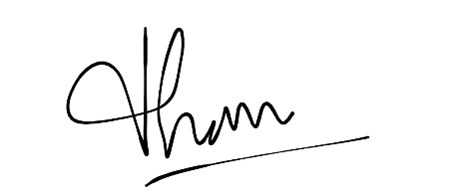
\includegraphics[width=3cm]{images/signature-dian.png}

\textbf{Dian Hanifudin Subhi, S.Kom., M.Kom.}

NIP. 198806102019031018
\end{flushright}

\clearpage

\section*{2. Anggota Peneliti 1}

\textbf{A. Identitas Diri}

{\footnotesize
\begin{longtable}{@{}p{0.8cm}p{6cm}p{0.3cm}p{8cm}}
1. & Nama Lengkap (dengan gelar) & : & Dika Rizky Yunianto, S.Kom., M.Kom. \\
2. & Jenis Kelamin & : & L \\
3. & Jabatan Fungsional & : & Asisten Ahli \\
4. & NIK & : & 3507220606920001 \\
5. & NIP & : & 199206062019031017 \\
6. & Tempat dan Tanggal Lahir & : & Malang, 06 Juni 1992 \\
7. & e-mail & : & dika.rizky@polinema.ac.id \\
8. & Nomor Telepon/HP & : & 081944819792 \\
9. & Alamat Kantor & : & Jl. Soekarno Hatta 09, Malang \\
10. & Nomor Telepon/Fax (kantor) & : & (0341) 404424, 404425 \\
11. & Lulusan yg telah dihasilkan & : & 40 orang \\
12. & Mata Kuliah yg diampu & : & Basis Data, Data Warehouse, Data Mining \\
\end{longtable}
}

\textbf{B. Riwayat Pendidikan}

{\footnotesize
\begin{longtable}{|p{3.5cm}|p{5cm}|p{5cm}|p{1.5cm}|}
\hline
& \textbf{S-1} & \textbf{S-2} & \textbf{S-3} \\
\hline
Nama Perguruan Tinggi & Universitas Brawijaya & Institut Teknologi Sepuluh Nopember Surabaya & - \\
\hline
Bidang Ilmu & Teknik Informatika & Teknik Informatika & - \\
\hline
Tahun Masuk-Lulus & 2010-2014 & 2015-2017 & - \\
\hline
Judul Skripsi/Tesis/Disertasi & Segmentasi Citra X-Ray Dental Bitewing Untuk Menentukan Jenis Gigi & Pengembangan Thesaurus Bahasa Arab berbasis Co-Occurence & - \\
\hline
Nama Pembimbing/Promotor & Dr. Candra Dewi, S.Kom., M.Sc & Prof. Dr. Agus Zainal Arifin, S.Kom., M.Kom & - \\
\hline
\end{longtable}
}

\textbf{C. Pengalaman Penelitian Dalam 10 Tahun Terakhir}

{\footnotesize
\begin{longtable}{|c|c|p{6.5cm}|c|c|c|}
\hline
\textbf{No} & \textbf{Tahun} & \textbf{Judul Penelitian} & \textbf{Sebagai} & \multicolumn{2}{c|}{\textbf{Pendanaan}} \\
\cline{5-6}
& & & & \textbf{Sumber} & \textbf{Jumlah (Rp)} \\
\hline
1 & 2023 & ANALISIS SISTEM INFORMASI MONITORING UTILITY PERFORMANCE PADA PT. AIO & Anggota & Politeknik & 8,000,000 \\
\hline
2 & 2023 & APLIKASI REKOMENDASI MAHASISWA BERPRESTASI NON-AKADEMIK DI JURUSAN TEKNOLOGI INFORMASI & Anggota & Politeknik & 8,000,000 \\
\hline
3 & 2022 & PENCARIAN DOKUMEN BERBASIS NORMALISASI LEVENSTHEIN-SIMILARITY PADA APLIKASI JTI MEETING & Anggota & Politeknik & 8,000,000 \\
\hline
4 & 2022 & Inovasi Pembelajaran Hybrid tipe Project Based Learning pada Media Sosial Instagram Marketing & Anggota & Politeknik & 25,000,000 \\
\hline
5 & 2021 & AEGIS APLIKASI CHATBOT CUSTOMER SERVICE JURUSAN TEKNOLOGI INFORMASI & Anggota & Politeknik & 25,000,000 \\
\hline
\end{longtable}
}

\textbf{D. Pengalaman Pengabdian Dalam 10 Tahun Terakhir}

{\footnotesize
\begin{longtable}{|c|c|p{6.5cm}|c|c|c|}
\hline
\textbf{No} & \textbf{Tahun} & \textbf{Judul Penelitian} & \textbf{Sebagai} & \multicolumn{2}{c|}{\textbf{Pendanaan}} \\
\cline{5-6}
& & & & \textbf{Sumber} & \textbf{Jumlah (Rp)} \\
\hline
1 & 2023 & PEMBUATAN SISTEM INFORMASI PENGUMUMAN UNTUK SISWA DAN ORANG TUA DI MIN I KOTA MALANG & Anggota & Politeknik & 7,000,000 \\
\hline
2 & 2022 & SISTEM INFORMASI AKADEMIK BERBASIS WEBSITE DI KB/TK ALFATH BUNULREJO KOTA MALANG & Anggota & Politeknik & 7,000,000 \\
\hline
3 & 2021 & PELATIHAN PEMANFAATAN MICROSOFT OFFICE DAN ADMINISTRATOR OPENSID UNTUK APARATUR DESA TUMPAKOYOT & Anggota & Politeknik & 7,000,000 \\
\hline
\end{longtable}
}

\textbf{E. Pengalaman Publikasi Jurnal Ilmiah}

{\footnotesize
\begin{longtable}{|c|c|p{6cm}|p{3.5cm}|p{2.5cm}|}
\hline
\textbf{No} & \textbf{Tahun} & \textbf{Judul Jurnal Ilmiah} & \textbf{Nama Jurnal Ilmiah} & \textbf{Kategori Publikasi Jurnal Ilmiah} \\
\hline
1 & 2024 & Design And Building Of The Utility Performance Monitoring System At PT. XYZ With Brainstorming Method & International Journal of Health Engineering and Technology & Teknologi Informasi \\
\hline
2 & 2023 & Comparison of Relational Database Modeling Performance based on Number of Normalized Entities & SMARTICS Journal & Teknologi Informasi \\
\hline
3 & 2023 & Natural language processing based chatbot for customer support system on higher education institution & AIP Conference Proceedings & Teknologi Informasi \\
\hline
4 & 2018 & Geo-Sentiment Analysis as a Location-Based Opinion Analysis System on Public Opinion Data about Governor Candidates & International Journal of Engineering \& Technology & Teknologi Informasi \\
\hline
5 & 2018 & Brain signal classification using genetic algorithm for right-left motion pattern & International Journal of Advanced Computer Science and Applications & Teknologi Informasi \\
\hline
6 & 2017 & Pengembangan Sistem Otomatisasi AC dan Lampu Menggunakan Fuzzy dan Raspberry Pi & JURNAL INFOTEL & Teknologi Informasi \\
\hline
7 & 2017 & Perhitungan Kemiripan Term Co-occurence Berdasarkan Cluster Dokumen Untuk Pengembangan Thesaurus Bahasa Arab & JURNAL INFOTEL & Teknologi Informasi \\
\hline
8 & 2015 & Pembobotan Kata BerbasiS Preferensi Dan Hubungan Semantik Pada Dokumen Fiqih Berbahasa Arab & Jurnal Teknologi Informasi dan Ilmu Komputer & Teknologi Informasi \\
\hline
\end{longtable}
}

\textbf{F. Pengalaman HKI Dalam 10 Tahun Terakhir}

{\footnotesize
\begin{longtable}{|c|c|p{8cm}|p{3cm}|}
\hline
\textbf{No} & \textbf{Tahun} & \textbf{Judul} & \textbf{Jenis HKI} \\
\hline
1 & 2020 & Aplikasi Peringkasan Teks Otomatis Portal Berita Online & Hak Cipta \\
\hline
2 & 2023 & Aplikasi Jayanti & Hak Cipta \\
\hline
3 & 2023 & Aplikasi BPSense & Hak Cipta \\
\hline
\end{longtable}
}

\vspace{1cm}

\begin{flushright}
Malang, 22 Januari 2026

\vspace{0.5cm}

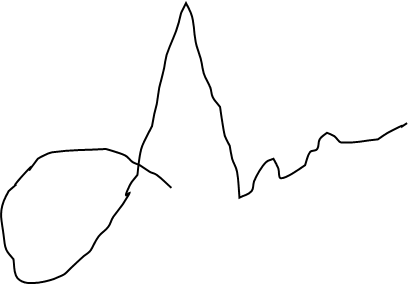
\includegraphics[width=3cm]{images/signature-dika.png}

\textbf{Dika Rizky Yunianto, S.Kom., M.Kom.}
\end{flushright}

\clearpage

\section*{3. Anggota Peneliti 2}

\textbf{A. Identitas Diri}

{\footnotesize
\begin{longtable}{@{}p{0.8cm}p{6cm}p{0.3cm}p{8cm}}
1. & Nama Lengkap & : & Ridwan Rismanto, S.ST., M.Kom., Ph.D. \\
2. & Jenis Kelamin & : & Laki-laki \\
3. & Jabatan Fungsional & : & Lektor \\
4. & NIP/NIK/Identitas Lainnya & : & 198603182012121001 \\
5. & NIDN & : & 0018038602 \\
6. & Tempat dan Tanggal Lahir & : & Malang, 18 Maret 1986 \\
7. & E-mail & : & rismanto@polinema.ac.id \\
8. & Nomor Telepon/HP & : & 085646313719 \\
9. & Alamat Kantor & : & Jl. Soekarno-Hatta 9 Malang \\
10. & Nomor Telepon/Faks & : & 0341-404424/0341-404420 \\
11. & Lulusan yang Telah Dihasilkan & : & D3=12; D4=35; S1= - ; S2= - ; S3= - \\
12. & Mata Kuliah yang diampu & : & Praktikum Dasar Pemrograman, Dasar Pemrograman, Struktur Data, Praktikum Struktur Data, Pemrograman Berbasis Objek, Praktikum Pemrograman Berbasis Objek, Metodologi Penelitian, Basis Data, Praktikum Basis Data, Sistem Pendukung Keputusan, Proyek Sistem Informasi, Data Science, Manajemen Korporasi \\
\end{longtable}
}

\textbf{B. Riwayat Pendidikan}

{\footnotesize
\begin{longtable}{|p{3cm}|p{3.5cm}|p{4cm}|p{3.5cm}|}
\hline
& \textbf{S-1} & \textbf{S-2} & \textbf{S-3} \\
\hline
Nama Perguruan Tinggi & Politeknik Elektronika Negeri Surabaya - ITS & Institut Teknologi Sepuluh Nopember & Hiroshima University \\
\hline
Bidang Ilmu & Teknologi Informasi & Teknik Informatika & Informatics and Data Science \\
\hline
Tahun Masuk -Lulus & 2004 – 2008 & 2009-2011 & 2021 - 2025 \\
\hline
Judul Skripsi/Thesis/Disertasi & Perancangan dan Pembuatan Aplikasi Keuangan Berbasis Web & Paralelisasi Transformasi Fourier Pada Arsitektur General Purpose Graphic Processing Unit Untuk Klasifikasi Alat Musik Dengan Instrumen Solo & A Study on Process Evaluation of Concept Map Recomposition \\
\hline
Nama Pembimbing & Isbat Uzzin N, S.Kom., MT. Siyamta, ST., MT. & Dr. Eng. Nanik Suciati, S.Kom., M.Kom. Wahyu Suadi, S.Kom., MM., M.Kom & Prof. Tsukasa Hirashima \\
\hline
\end{longtable}
}

\textbf{C. Pengalaman Penelitian dalam 5 Tahun Terakhir}

{\footnotesize
\begin{longtable}{|c|c|p{10cm}|c|}
\hline
\textbf{No.} & \textbf{Tahun} & \textbf{Judul Penelitian} & \textbf{Sumber} \\
\hline
1 & 2021 & Pengembangan Model Deteksi Lahan Parkir Kosong Menggunakan Metode Deep Learning (tugas belajar) & DIPA \\
\hline
\end{longtable}
}

\textbf{D. Pengalaman Penulisan Artikel Ilmiah dalam Jurnal dalam 5 Tahun Terakhir}

{\footnotesize
\begin{longtable}{|c|p{6cm}|p{3cm}|p{4cm}|}
\hline
\textbf{No.} & \textbf{Judul Artikel Ilmiah} & \textbf{Nama Jurnal} & \textbf{Volume/Nomor/Tahun} \\
\hline
1 & Identifikasi Pneumonia Pada Citra Rontgen Paru Menggunakan Metode Power-Law Trans & Jurnal Informatika Polinema 7 (2), 73-78 & Vol 7/No 2/ 2021 \\
\hline
2 & Sistem UMKM Online Produk Penjualan Kampoeng Sejarah Kota Malang Berbasis Website & Jurnal Pengabdian Polinema Kepada Masyarakat 8 (2), 102-104 & Vol 8/No 2/2021 \\
\hline
3 & Analysis of Comparison of Fuzzy Knn, C4. 5 Algorithm, and Naïve Bayes Classification Method for Diabetes Mellitus Diagnosis & International Journal of Computer Applications Technology and Research & Vol 7/No 8/2023 \\
\hline
4 & Experimental Evaluation of OOP Concepts Learning with a Kit-Build Concept Map: A Case Study & International Journal of Information and Education Technology 13 (9), 1358-1364 & Vol 13/No 9/2023 \\
\hline
5 & Evaluating the kit-build concept mapping process using sub-map scoring & Research and Practice in Technology Enhanced Learning & Vol 19/No 21/2024 \\
\hline
6 & The evaluation of concept map recomposition order and its effect on learning outcomes & Research and Practice in Technology Enhanced Learning & Vol 21/2026 \\
\hline
\end{longtable}
}

\textbf{E. Pemakalah Seminar Ilmiah (Oral Presentation) dalam 5 Tahun Terakhir}

{\footnotesize
\begin{longtable}{|c|p{5.5cm}|p{5cm}|p{3.5cm}|}
\hline
\textbf{No.} & \textbf{Nama Pertemuan Ilmiah/Seminar} & \textbf{Judul Artikel} & \textbf{Waktu dan Tempat} \\
\hline
1 & A Preliminary Study: Toulmin Arguments in English Reading Comprehension for English as Foreign Language Students & 2021 International Conference on Electrical and Information Technology & September 2021, Malang, Indonesia \\
\hline
2 & Rekomendasi e-Book pada Digital Repository Rumah Sakit Umum Universitas Kristen Indonesia dengan menggunakan Metode VIKOR & Seminar Informatika Aplikatif Polinema & November 2021, Malang, Indonesia \\
\hline
3 & Process Evaluation for Concept Map Building and Its Experimental Evaluation & International Conference on Computers in Education & Desember 2023, Shimane, Jepang \\
\hline
4 & Trial-and-Error Modifications as Cognitive Compensation: Analyzing the Concept Mapping Process in Reconstruction Tasks & International Conference on Computers in Education & Desember 2025, Chennai, India \\
\hline
\end{longtable}
}

\textbf{F. Perolehan HKI dalam 5 – 10 Tahun Terakhir}

{\footnotesize
\begin{longtable}{|c|p{8cm}|c|c|c|}
\hline
\textbf{No.} & \textbf{Judul/Tema HKI} & \textbf{Tahun} & \textbf{Jenis} & \textbf{Nomor P/ID} \\
\hline
1 & Program Rekomendasi Artikel Terkait Pada Berita Online Menggunakan Teknik Text Mining (tugas belajar) & 2019 & Program Komputer & EC00201977365 \\
\hline
\end{longtable}
}

\vspace{0.5cm}

\noindent
Semua data yang saya isikan dan tercantum dalam biodata ini adalah benar dan dapat dipertanggung jawabkan secara hukum. Apabila di kemudian hari ternyata dijumpai ketidaksesuaian dengan kenyataan, saya sanggup menerima sanksi. Demikian biodata ini saya buat dengan sebenarnya untuk memenuhi salah satu persyaratan dalam Penelitian dan Pengabdian Masyarakat.

\vspace{1cm}

\begin{flushright}
Malang, 25 Januari 2026

\vspace{0.5cm}

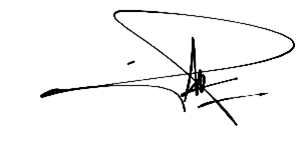
\includegraphics[width=3cm]{images/signature-ridwan.png}

\textbf{Ridwan Rismanto, S.ST., M.Kom., Ph.D.}

NIP. 198603182012121001
\end{flushright}

\clearpage

\section*{4. Anggota Peneliti 3}

\textbf{A. Identitas Diri}

{\footnotesize
\begin{longtable}{@{}p{0.8cm}p{6cm}p{0.3cm}p{8cm}}
1. & Nama Lengkap (dengan gelar) & : & Usman Nurhasan, S.Kom., M.T \\
2. & Jenis Kelamin & : & Laki-laki \\
3. & Jabatan Fungsional & : & Lektor \\
4. & NIP/NIK/No. identitas lainnya & : & 198609232015041001 \\
5. & NIDN & : & 0023098604 \\
6. & Tempat dan Tanggal Lahir & : & Malang, 23 September 1986 \\
7. & E-mail & : & usmannurhasan@polinema.ac.id \\
8. & Nomor Telepon/HP & : & 082143246664 \\
9. & Alamat Kantor & : & Jl. Soekarno Hatta no. 9 Malang 65141 \\
10. & Nomor Telepon/Faks & : & 0341-404424 \\
11. & Mata Kuliah yg Diampu & : & Multimedia Terapan, Pemrograman Jaringan, Aplikasi Enterprise, Jaringan Komputer, Sistem Operasi \\
\end{longtable}
}

\textbf{B. Riwayat Pendidikan}

{\footnotesize
\begin{longtable}{|p{3.5cm}|p{5.5cm}|p{6cm}|}
\hline
& \textbf{S-1} & \textbf{S-2} \\
\hline
Nama Perguruan Tinggi & Universitas Islam Negeri Maulana Malik Ibrahim Malang & Universitas Brawijaya Malang \\
\hline
Bidang Ilmu & Teknik Informatika & Teknik Elektro Minat Sistem Komunikasi dan Informatika \\
\hline
Tahun Masuk- Lulus & 2005-2010 & 2011-2014 \\
\hline
Judul Skripsi/ Tesis/Disertasi & Rancang Bangun Aplikasi Pengontrol Peralatan Listrik Menggunakan NM7010 Adan DT-AVR Low Cost Series & Sistem Cerdas Pencarian Lokasi Parkir Terbaik dengan Algoritma Fuzzy-Best Fit \\
\hline
Nama Pembimbing/ Promotor & 1. Totok Chamidy, S.Kom., M.Kom 2. Dr. Ahmad Barizy, M.Ag & 1. Hadi Suyono, ST., MT., Ph.D 2. Dr. Aziz Muslim, MT \\
\hline
\end{longtable}
}

\textbf{C. Pengalaman Penelitian Dalam 5 Tahun Terakhir}

{\footnotesize
\begin{longtable}{|c|c|p{6cm}|c|c|}
\hline
\textbf{No.} & \textbf{Tahun} & \textbf{Judul Penelitian} & \textbf{Sumber*} & \textbf{Jml (Juta Rp)} \\
\hline
1 & 2016 & Sistem Cerdas Tes Psikologi Papi Kostick Untuk Seleksi Masuk Mahasiswa Baru Jalur D-III Kerjasama Polinema Dengan PLN Dan PT GMF Aeroasia & DIPA & 4 \\
\hline
2 & 2016 & Pengembangan Sistem Analisa Sentimen Pada Kata Kunci Tertentu Di Dalam Sebuah Korpus Teks & DIPA & 4 \\
\hline
3 & 2017 & Implementasi Fuzzy Inference System Pada Sistem Cerdas Tes Psikologi Kraepelin & DIPA & 4 \\
\hline
4 & 2017 & Sistem Cerdas Penentu Rekomendasi Pemilihan Jalur Angkot Kota Malang & DIPA & 4 \\
\hline
5 & 2018 & Efektifitas Mobile Art Application (MATA) Sebagai Media Penanganan Kasus Agresi Pada Anak & DIPA & 4 \\
\hline
6 & 2018 & Implementasi Teksturing Secara Real Time Pada Augmented Reality (AR) & DIPA & 4 \\
\hline
7 & 2018 & Implementasi Smart Mirror Tracer Untuk Mendeteksi Tingkat Dominan dan Emosi & DIPA & 25 \\
\hline
8 & 2019 & Penerapan Teknologi Hybrid (Augmented Reality Dan Geographic Information System) Untuk Tourist Guide Application & DIPA & 8 \\
\hline
9 & 2019 & Perancangan Game Edukasi Pengenalan Huruf Hijaiyah Untuk Anak Berbasis Augmented Reality & DIPA & 8 \\
\hline
10 & 2019 & Aplikasi Pembelajaran Bahasa Inggris Berbasis Augmented Reality & DIPA & 8 \\
\hline
11 & 2019 & Pemanfaatan Konten Virtual Reality Untuk Simulasi Matakuliah Praktikum & DIPA & 50 \\
\hline
12 & 2020 & Implementasi E-Reporting Infrastructure (Eri) Sebagai Media Monitoring Kerusakan Infrastruktur Dalam Kampus & DIPA & 8 \\
\hline
13 & 2020 & Smart Ecosystem Untuk Lahan Hidroponik Pada Kelompok Petani Hidroponik Binaan CSR PT. Otsuka Indonesia Sebagai Peningkatan Kualitas Dan Kuantitas Hasil Panen & DIPA & 70 \\
\hline
14 & 2021 & Implementasi Sistem Cerdas Eksperimen Gambar Untuk Analisis Kondisi Adversity Response Profile (ARP) & DIPA & 8 \\
\hline
\end{longtable}
}

\textbf{D. Pengalaman Pengabdian Kepada Masyarakat dalam 5 Tahun Terakhir}

{\footnotesize
\begin{longtable}{|c|c|p{6cm}|c|c|}
\hline
\textbf{No.} & \textbf{Tahun} & \textbf{Judul Pengabdian Kepada Masyarakat} & \textbf{Sumber*} & \textbf{Jml (Juta Rp)} \\
\hline
1. & 2016 & Penerapan Sistem Pengawasan IP Camera di Yayasan Pendidikan Islam & DIPA & 3,6 \\
\hline
2 & 2017 & Pelatihan Pengolahan Nilai Raport kepada Guru di SDN 1 Sukun Kota Malang & DIPA & 3,6 \\
\hline
3 & 2018 & Packaging dan Promosi Produk Bahan Olahan Makanan Untuk Meningkatkan Daya Saing (Studi Kasus UKM "Makanan Olahan Menuk") & DIPA & 3,6 \\
\hline
4 & 2019 & Pelatihan Pemanfaatan Aplikasi Smart.04 & DIPA & 6,8 \\
\hline
5 & 2019 & Pelatihan Keterampilan Dasar Komputer Dan Pengolahan Nilai Raport Bagi Guru Smp Islam Al-Amin Kota Malang & DIPA & 6,8 \\
\hline
6 & 2020 & Pelatihan Pemanfaatan Marketplace Tani-Ku Sebagai Media Promosi Dan Transaksi Bagi Penggiat Hidroponik Di Kota Batu & DIPA & 6,8 \\
\hline
7 & 2020 & Pelatihan Keterampilan Dasar Komputer Dan Tata Kelola Organisasi Pada Komunitas Pemuda Penggiat Sejarah Di Kelurahan Sumbersari Kota Malang & DIPA & 6,8 \\
\hline
8 & 2020 & Sosialisasi Pentingnya Literasi Digital Untuk Meningkatkan Komunikasi Digital Bagi Komunitas Reenactor Ngalam & DIPA & 6,8 \\
\hline
9 & 2021 & Pelatihan Pemanfaatan Media Literasi Mandiri Di Lingkungan Madrasah Aliyah Negeri 1 Malang Sebagai Usaha Mewujudkan Smart School & DIPA & 7 \\
\hline
\end{longtable}
}

\textbf{E. Publikasi Artikel Ilmiah Dalam Jurnal dalam 5 Tahun Terakhir}

{\footnotesize
\begin{longtable}{|c|p{5.5cm}|p{5cm}|p{3cm}|}
\hline
\textbf{No.} & \textbf{Judul Artikel Ilmiah} & \textbf{Nama Jurnal} & \textbf{Volume/ Nomor/Tahun} \\
\hline
1 & Sistem Cerdas Pencarian Lokasi Parkir Terbaik dengan Algoritma Fuzzy-Best Fit & Electrical Power, Electronics, Communications, Controls, and Informatics (EECCIS) & Volume 8 / No 1 / Tahun 2014 \\
\hline
2 & Sistem Cerdas Papi Kostick & JURNAL TEKNO LOGI INFORMASI: Teori, Konsep, dan Implementasi ISSN : 2086 - 2989 & Volume 12/ No 1 /Tahun 2017 \\
\hline
3 & Sistem Cerdas Tes Kepribadian Kraepelin & JURNAL TEKNO LOGI INFORMASI: Teori, Konsep, dan Implementasi ISSN : 2086 - 2989 & Volume 8 / No. 2/ 2017 \\
\hline
4 & Sistem Cerdas Penentu Rekomendasi Pemilihan Jalur Angkot Kota Malang & Jurnal ANTIVIRUS :Jurnal Ilmiah Teknik Informatika ISSN 1978-5232 & Volume 11/ Tahun 2017 \\
\hline
5 & Implementation IoT in System Monitoring Hydroponic Plant Water Circulation and Control & International Journal of Engineering and Technology(UAE) ISSN: 2227-524X & Volume 7/2018 \\
\hline
6 & Realtime Mobile Queue System Multi Vendor & Jurnal Informatika Polinema ISSN: 2614-6371 & Volume 5/Tahun 2019 \\
\hline
7 & Pemanfaatan Website Untuk Manajemen Informasi Penelitian Peternakan Kota Batu & Jurnal Antivirus: Jurnal Ilmiah Teknik Informatika ISSN 1978-5232 & Volume 13/Tahun 2019 \\
\hline
8 & Perancangan Sistem Informasi Pengolahan Data Belanja Langsung Berbasis Website & Generation Journal e-ISSN number: 2549-2233 p-ISSN: 2580-4952 & Volume 3 / Tahun 2019 \\
\hline
9 & Simulasi Virtual Reality Pendeteksi Tingkat Phobia Seseorang Sebagai Alat Bantu Terapi Acrophobia (Phobia Ketinggian) Berbasis Android & Jurnal Informatika Polinema ISSN: 2614-6371 & Volume 5/Tahun 2019 \\
\hline
10 & Sistem Informasi Geografis Pencarian Jalur Terdekat Desa Wisata Studi Kasus Kota Wisata Batu & Jurnal Informatika Polinema ISSN: 2614-6371 & Volume 5/Tahun 2019 \\
\hline
11 & Mobile Art Application (MATA) as a media for handling cases of aggression in children & Journal of Physics: Conference Series & 1402 (6), 066049, 2019 \\
\hline
12 & Study of image reconstructions of Indonesian traffic sign using Criminisi and Hung method & Journal of Physics: Conference Series & 1402 (6), 066032 \\
\hline
13 & "Hijaiyah" interactive learning for pre-school students & Journal of Physics: Conference Series & 1402 (6), 066050 \\
\hline
14 & Smart tourist guide application for the introduction of Malang city tourism potential using hybrid technology & Journal of Physics: Conference Series & 1402 (6), 066051 \\
\hline
15 & Utilization of virtual reality content for laboratory practicum learning & IOP Conference Series: Materials Science and Engineering & 732 (1), 012087/ 2020 \\
\hline
16 & Pengembangan Aplikasi Deteksi Dini Pada Anak Berkebutuhan Khusus Di Sekolah Luar Biasa & Petir: Jurnal Pengkajian dan Penerapan Teknik Informatika & 14 (1), 17-27/ 2020 \\
\hline
17 & Implementasi Metode MVC Untuk Pembangunan Sistem Informasi Pelatihan Kerja: Studi Kasus UPT Pelatihan Kerja Singosari & Jurnal Eksplora Informatika & 10 (1), 20-31 1/ 2020 \\
\hline
18 & Pembelajaran Humane Education Di Kurikulum 2013 Menggunakan Media Animasi & Urbangreen Conference Proceeding Library & 1, 176-182/ 2020 \\
\hline
19 & Analisis Perilaku Non Playable Character (Npc) Pada Game Menggunakan Fuzzy Sugeno & Techno. Com & 19 (3), 308-320/ 2020 \\
\hline
20 & Penerapan Aplikasi Up-Event Pada Tata Kelola Kegiatan Multi Vendor & Generation Journal & 4 (2), 84-97 \\
\hline
21 & Pemodelan Konten Augmented Reality Dalam Konsep Interactive Realtime & Jurnal Informatika & 20 (1), 30-40/2020 \\
\hline
22 & Media Pembelajaran Interaktif Terhadap Gwk Culture Park Menggunakan Teknologi Augmented Reality & Jurnal Informatika Polinema & 6 (3), 1-8/2020 \\
\hline
23 & Implementation of Hybrid Methods in the Application of Experimental Psychology for Analysis of Mental Endurance Conditions & Khazanah Informatika: Jurnal Ilmu Komputer dan Informatika 7 (1) & Vol 7/ No 1/2021 \\
\hline
24 & Mobile Media Literature Application For Identification Of Student's Reading Interest & Jurnal Riset Informatika (JRI) & Vol 3 No 4 (2021): Period of September 2021 \\
\hline
25 & Penerapan Vector Space Model Dalam Klasifikasi Penilaian Thematic Appeception Test & J-SAKTI (Jurnal Sains Komputer \& Informatika) & Vol 5, No 2 / 2021 \\
\hline
26 & Implementasi Metode Fuzzy Time Series Markov Chain untuk Prediksi Harga Telur Puyuh & Informatika Mulawarman : Jurnal Ilmiah Ilmu Komputer & Vol 16, No 2/2021 \\
\hline
\end{longtable}
}

\textbf{F. Pemakalah Seminar Ilmiah (Oral Presentation) dalam 5 Tahun Terakhir}

{\footnotesize
\begin{longtable}{|c|p{5cm}|p{5.5cm}|p{3.5cm}|}
\hline
\textbf{No.} & \textbf{Nama Temu ilmiah/Seminar} & \textbf{Judul Artikel Ilmiah} & \textbf{Waktu dan Tempat} \\
\hline
1 & MATEC Web of Conferences & The evaluation on a mobile augmented reality application as therapy media & 2018, Bandung, Jawa Barat, Indonesia \\
\hline
2 & Proceedings of the 2018 International Conference on Energy and Mining Law (ICEML 2018) & Analysis of Sand Mining Areas in Lumajang Using WEBGIS & 2018, Bandung, Jawa Barat, Indonesia \\
\hline
3 & The 4th Annual Applied Science and Engineering Conference & Mobile Art Application (MATA) as a media for handling cases of aggression in children & 2019, Bali, Indonesia \\
\hline
4 & The 4th Annual Applied Science and Engineering Conference & Study of image reconstructions of Indonesian traffic sign using Criminisi and Hung method & 2019, Bali, Indonesia \\
\hline
5 & The 4th Annual Applied Science and Engineering Conference & "Hijaiyah" interactive learning for pre-school students & 2019, Bali, Indonesia \\
\hline
6 & The 4th Annual Applied Science and Engineering Conference & Smart tourist guide application for the introduction of Malang city tourism potential using hybrid technology & 2019, Bali, Indonesia \\
\hline
7 & Seminar Nasional Terapan Riset Inovatif (Sentrinov) 2019 & Penerapan Socket Programming Pada Game Multi Client "Di Kejar Musuh" & 2019, Bangka Belitung, Indonesia \\
\hline
8 & Seminar Nasional Terapan Riset Inovatif (Sentrinov) 2019 & Pemanfaatan Konten Virtual Reality Sebagai Media Terapi Penderita Ophidiophobia & 2019, Bangka Belitung, Indonesia \\
\hline
9 & The 2nd International Conference on Applied Science and Technology (iCAST) 2019, & Implementation of Augmented Reality For Autism Children Therapy Spectrum Disorder & 2019, Bali, Indonesia \\
\hline
10 & The 2nd Annual Technology, Applied Science and Engineering Conference (ATASEC 2020) & Smart Ecosystem For Hydroponic Land In The Hydroponic Farmers Group Guided By CSR PT. Otsuka Indonesia As An Improved Quality And Quantity Of Harvest Results & 2020, Indonesia \\
\hline
11 & Seminar Nasional Psikologi UM (2021) & Problematika Pembelajaran Jarak Jauh (PJJ) Mata Pelajaran Informatika pada Masa Pandemi di MAN 1 Kota Malang & 2021, Malang \\
\hline
12 & UrbanGreen Conference Proceeding Library & Pembelajaran Humane Education di Kurikulum 2013 Menggunakan Media Animasi & 2021, Malang \\
\hline
13 & International Conference on Industrial Revolution for Polytechnic Education & Application of WebSocket on Integration of E-Reporting Infrastructure (ERI) Applications with IoT & 2021, Malang \\
\hline
\end{longtable}
}

\textbf{G. Karya Buku dalam 5 Tahun Terakhir}

{\footnotesize
\begin{longtable}{|c|p{7cm}|c|c|p{2.5cm}|}
\hline
\textbf{No.} & \textbf{Judul Buku} & \textbf{Tahun} & \textbf{Jumlah Halaman} & \textbf{Penerbit} \\
\hline
1 & Pemrograman Jaringan Menggunakan Java Jilid 1 & 2018 & 107 & Polinema Press \\
\hline
2 & Pemrograman Jaringan Menggunakan Java Jilid 2 & 2018 & 260 & Polinema Press \\
\hline
3 & Isu Profesional dan Sosial di Bidang IT & 2019 & 132 & Polinema Press \\
\hline
4 & Pengantar Sistem Operasi dan Remastering Linux & 2020 & 174 & Polinema Press \\
\hline
5 & Pengantar Rekayasa Perangkat Lunak & 2020 & 190 & Polinema Press \\
\hline
\end{longtable}
}

\textbf{H. Perolehan HKI dalam 10 Tahun Terakhir}

{\footnotesize
\begin{longtable}{|c|p{6cm}|c|c|c|}
\hline
\textbf{No.} & \textbf{Judul/Tema HKI} & \textbf{Tahun} & \textbf{Jenis} & \textbf{Nomor P/ID} \\
\hline
1 & ARDoa Augmented Reality Doa & 2018 & Hak Cipta & EC00201858687 \\
\hline
2 & Media Pembelajaran Berbasis Animasi "Animal Education" & 2019 & Hak Cipta & EC00201983866 \\
\hline
3 & E-Reporting Infrastruktur (ERI) Kampus & 2020 & Hak Cipta & EC00202044987 \\
\hline
4 & Aplikasi Marketplace Tani-Ku & 2020 & Hak Cipta & EC00202044986 \\
\hline
5 & Art Drawing Sebagai Media Komunikasi Nonverbal & 2020 & Hak Cipta & EC00202044046 \\
\hline
6 & Aplikasi E-Payment Bank Sampah & 2020 & Hak Cipta & EC00202044045 \\
\hline
7 & ARSurya : Aplikasi Media Pembelajaran Tat Surya Berbasis Augmented Reality & 2020 & Hak Cipta & EC00202044044 \\
\hline
\end{longtable}
}

\vspace{0.5cm}

\noindent
Semua data yang saya isikan dan tercantum dalam biodata ini adalah benar dan dapat dipertanggungjawabkan secara hukum. Apabila di kemudian hari ternyata dijumpai ketidak-sesuaian dengan kenyataan, saya sanggup menerima risikonya.

\noindent
Demikian biodata ini saya buat dengan sebenarnya untuk memenuhi salah satu persyaratan dalam pengajuan penelitian dan pengabdian.

\vspace{1cm}

\begin{flushright}
Malang, 25 Januari 2026

\vspace{0.5cm}


\includegraphics[width=3cm]{images/signature-usman.png}

\textbf{Usman Nurhasan, S.Kom., M.T}

NIP. 198609862015041001
\end{flushright}

\clearpage

\addcontentsline{toc}{chapter}{D. SURAT PERNYATAAN KEASLIAN}

\vspace*{-2cm}
\noindent
\makebox[\textwidth][c]{%
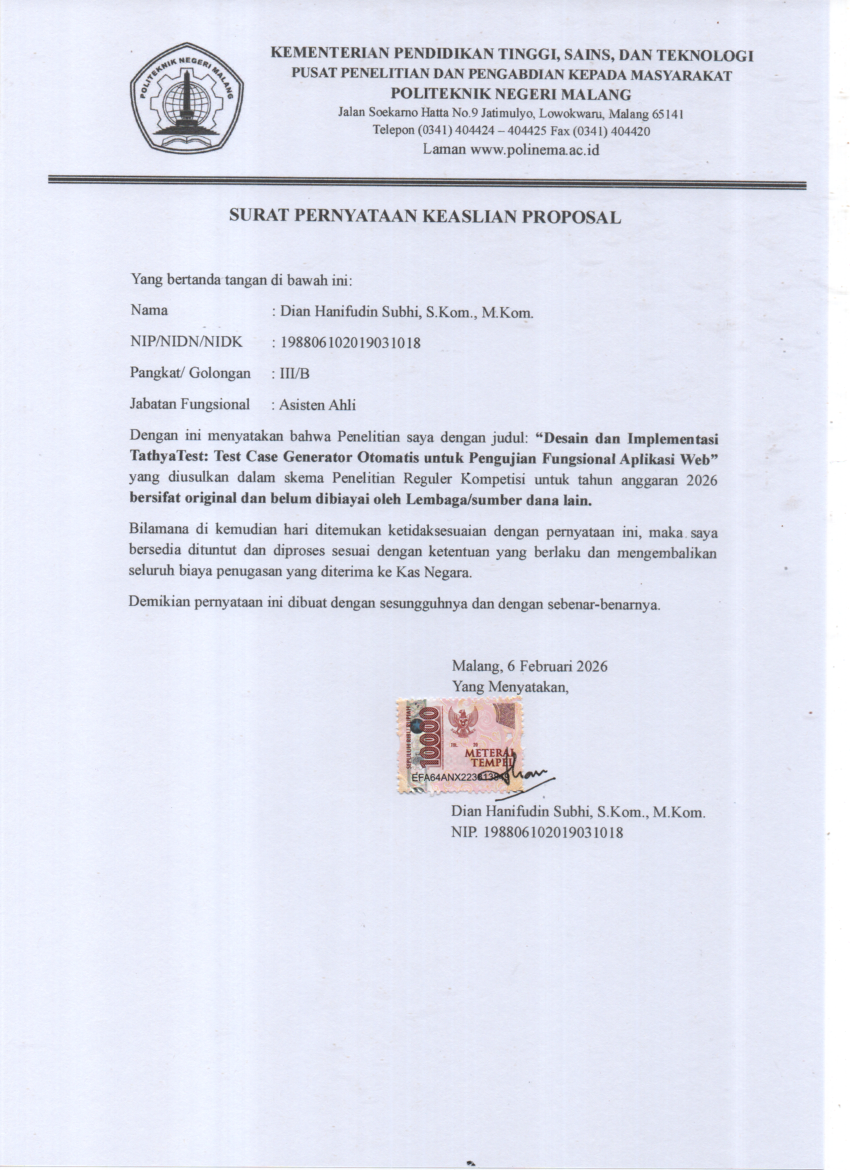
\includegraphics[width=1.2\textwidth,keepaspectratio]{images/surat-pernyataan-keaslian.png}
}


\end{document}
